% -------------------------------
% == REPORT 2 ==
% -------------------------------
% -------------------------------
% Madison: Odd numbered sections
% Jake: Even numbered sections
% -------------------------------
% -------------------------------
%

\documentclass[conf]{new-aiaa}

\usepackage[utf8]{inputenc}
\usepackage{float}
\usepackage{graphicx}
\usepackage{amsmath}
\usepackage[version=4]{mhchem}
\usepackage{siunitx}
\usepackage{longtable,tabularx}
\setlength\LTleft{0pt} 
\usepackage{hyperref}
\usepackage{nomencl}
\usepackage{lscape}

\linespread{2}  

\title{Design Report 02: Twin Sea Lion}

\author{
    Madison Junker\footnote{Student ID: 102736535 }, Jacob Killelea\footnote{Student ID: 10550162 } \\
    \emph{ASEN 4138, University of Colorado Boulder, October 26, 2018}
}

\begin{document}

\clearpage
\maketitle
\thispagestyle{empty}

\newpage
\pagenumbering{roman}
\tableofcontents
\addcontentsline{toc}{section}{\listfigurename}
\listoffigures
\addcontentsline{toc}{section}{\listtablename}
\listoftables
\newpage
\printnomenclature[25mm]

\section*{Nomenclature}

{\renewcommand\arraystretch{1.0}
\noindent\begin{longtable*}{@{}l @{\quad=\quad} l@{}}
$AAA$     	               & Advanced Aircraft Analysis Program \\
$AR_W$    	               & Aspect Ratio                       \\
$b_W$	  	               & Wing Span                          \\
$\bar{c}_W$	  	           & Mean Geometric Chord               \\
$i_W$		               & Incidence Angle                    \\
KTAS                       & Knots True Airspeed                \\
$l_f$     	               & Length of fuselage                 \\
$MSL$     	               & Mean Sea Level Altitude            \\
$S_W$     	               & Wing Area                          \\
$TWR$     	               & Thrust to weight ratio             \\
$\epsilon_W$               & Wing Twist Angle                   \\
$\Lambda_{c/4w}$[$^\circ$] & Wing Sweep Angle                   \\
$\lambda_W$	               & Taper Ratio                        \\
$\lambda_{c/4w}$           & Quarter-chord Sweep Angle          \\
$\Gamma_W$	               & Dihedral                           \\
\end{longtable*}}

\newpage
\pagenumbering{arabic}

% 1
\section{Introduction}
% The Twin Sea Lion is a combination cargo and transport plane designed to transport a small number of 
The Twin Sea Lion is an upcoming cargo and personal transport aircraft meant for moving payloads over 1500 nautical miles quickly and efficiently. The aircraft is designed with challenging airports in mind, with planned takeoffs and landings from Aspen Airport, a 4000 foot runway at 7000 feet MSL. At lower altitudes, this equates to STOL performance. It has a takeoff weight of 37,689 pounds and a useful load of 16,682 pounds. Pratt and Whittney PW150A turboprop engines provide exceptional power and economy of operation. This report presents design considerations including the cockpit and cabin layouts, wing geometry and planform, flap configuration, and engine power calculations.

% 2
\section{Addendum to Report 1}

\begin{figure}[H]
    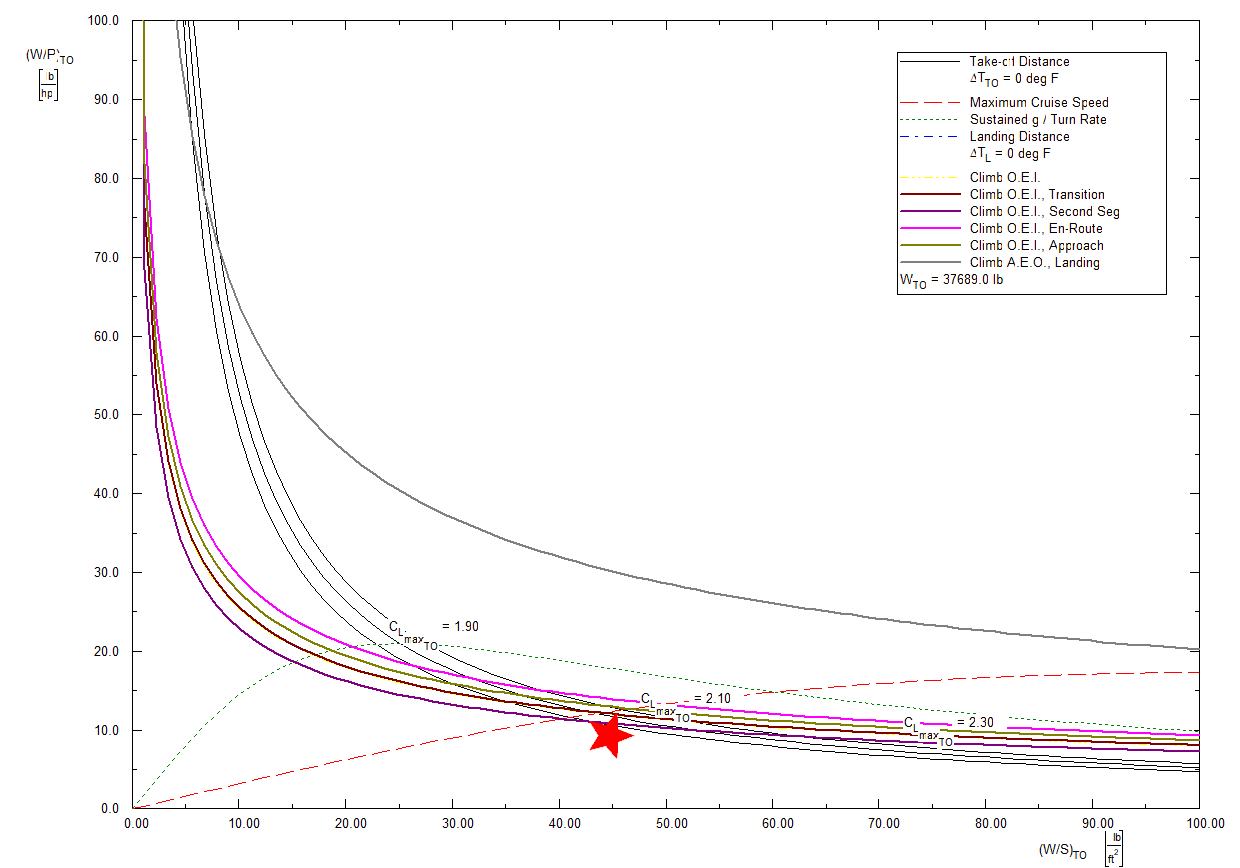
\includegraphics[width=\textwidth]{plots/new_perf_sizing_annotated}
    \caption{Revised performance sizing plots}
    \label{fig:new_perf_sizing}
\end{figure}

In Design Report 1, takeoff and maneuvering performance sizing plots were misinterpreted. Original 
performance sizing plots showed much lower lines for cruise and maneuvering performance constraints 
and a design point above these lines was chosen. This proved to be incorrect, however, as all example plots were given for a jet aircraft and the y-axis of the plot was thrust to weight (TWR). This plot shows power loading, so all the lines that the aircraft would need to be above, it now must be below. Cruise and maneuvering constraints were raised by decreasing the cruise speed from 0.8 to 0.6 Mach. Thankfully, this did not appreciably change the design point and wing loading was kept at roughly 45 pound per square foot and power loading at 8 pounds per horsepower, leading to a power requirement of 4711 total horsepower.

% 3
\section{Configuration Selection}
\subsection{Selection of the Overall Configuration}
%Describe how you chose the configuration for your aircraft and why
A conventional configuration will provide the most reliable performance for the Twin Sea Lion. The Sea Lion needs large wings and engines to meet its STOL goal and thus large wings to produce lift and place engines. As the Sea Lion will be following a standard transport mission profile, there is no need for greater maneuverability as may be provided by a canard or Mach cone avoidance as provided by a Delta wing. A conventional wing provides high amounts of structural strength and space for the high-lift devices necessary for STOL. Though a conventional wing may not be at the forefront of all possible aerodynamics, this small disadvantage does not outweigh the advantages.

\subsection{Wing Bracing and Position}
%Is the wing braced (with struts) or cantilever? why?
%Low wing, high wing or mid wing mount to fuselage? Explain
The Sea Lion wings will be cantilevered. With a cruise Mach number of 0.6, the drag from wing struts would be extremely large.

A low mounted wing would reduce the gear length and weight and keep the wingbox out of the way. However, this decreases the possible size of the propellers. The powerful engines planned for the Twin Sea Lion will need comparably large propellers, so this point needs special attention. A mid mounted wing would allow more room for propellers but would require longer gears and puts the wing box in the middle of the plane. This would interfere with passenger comfort should the cargo to passenger proportion not allow for separation of cargo and passenger area with the wingbox. A high mounted wing would allow for the largest propellers but would require the gears to be in the fuselage to avoid extreme gear weight.

The British Aerospace ATP used a low mounted wing and large propellers by mounting the engines above the wings. Since the wing volume for our plane is much larger than needed for fuel with a relatively thin airfoil, the wing also makes the best position for the main landing gear. Therefore, the Twin Sea Lion will use a low mounted wing.

% 4
\section{Fuselage and Cockpit Layout Design}
\subsection{Fuselage and Cabin Layout Design}
% You should include well-dimensioned and labeled fuselage/cabin layout drawings (top and side views) and a fuselage/cabin cross-section drawing in this section. Drawing must be done using a drawing program. Drawings should include furnishing, aisles, and exits. Discuss your layout, why did you place items where you did? Do you satisfy all regulatory egress requirements? Does all the baggage/cargo fit? Where is it located? Also include you fineness ratio (lf/df) as well as (We/lf) values and compare with similar aircraft

Fuselage width was determined from seat width, aisle width, and estimates for wall width. With 10 passengers, the Sea Lion needs 15 inches of aisle. Though an aisle width of 20 inches may be more suitable for embarking and disembarking, this narrow aisle will allow for wider seats and thus more comfort for sitting passengers, which will account for most of the flight. De Luxe Seats (Table 3.1, Pres 11) have 20 inches of cushion width and 2.75 inches for armrests. With two armrests a seat and two seats in a row across the fuselage, this is 51 inches for seats and 66 inches wide total in the interior. However, given considerations for headroom of the occupants, the inner diameter of the cabin was increased to 76 inches. Total exterior diameter is 8\% larger than interior diameter, which puts exterior diameter at 82 inches.

Space between seat was determined by the femur length of a member of the design team, plus one inch for a $q1$ total of 25 inches. This gives a row width of 50.5 inches, including the existing 25.5 seat length.

The lavatory was chosen to match the dimensions of the lavatory in the Gulfstream I as in Table 3.6 of presentation 12 \cite{pres12} since this plane was of comparable passenger number. No galley or wardrobe were deemed necessary for this trip length.

Necessary cargo dimensions were determined from assumptions of bag density of $12.5 lb/ft^3$ and packing efficiency of 85\%. With 2400 pounds of cargo this equates to $225.88 ft^3$. With a removable aisle floor, some cargo can fit under the seat.  The usable volume of this space was estimated as a trapezoid stretched below all passenger seats as depicted in figure \ref{fig:fuselage_annotated}. Thus the volume is $(20.5in\cdot 17.55in)+(22.63in\cdot 17.55in)=181,663in^3=105.129ft^3$. The next most available space is across from the lavatory. This was also estimated as a trapezoid as in figure \ref{fig:fuselage_annotated} stretched along the length of the lavatory. This volume is $(20.86in\cdot 17.01in)+(38.05in\cdot 20.86in)=60,870in^3=35.23ft^3$. This leaves $115.523ft^3$ remaining. The final cargo space was assumed to take the entire interior fuselage cross sectional area ($A=\frac{1}{4}\pi(75.97/12ft)^2=31.478ft^2$) and had a length determined from $\frac{115.523ft^3}{31.478ft^2}=3.67 ft = 44.04 in$. An inch was added to allow for a wall between this main cargo area and the passenger area. 

\begin{table}[H]
\centering
\caption{Characteristics of similar airplanes}
\label{tab:similarplanes}
\begin{tabular}{|c|c|c|c|c|c|} \hline
Plane & $l_f$ [ft] & $d_f$ [ft] & $W_E$ [lb] & $W_E/l_f$ & $l_f/d_f$\\ \hline
 DHC-6 Twin Otter & 51.74 & 5.75& 7,100  & 137.23 & 9.0 \\ \hline
 PC-24            & 55.12 & 5.6	& 10,957 & 198.79 & 9.8\\ \hline
 DHC-4 Caribou    & 73.98 & 6.125	& 16,920 & 228.70 & 12.1 \\ \hline
 F-27 Friendship  & 77.30 & 	& 27,964 & 361.78 & \\ \hline
 Dash 8 Q-400     & 107.74 & 8.25	& 36,520 & 338.96 & 13.1\\ \hline
 Twin Sea Lion	& 47.58 & 6.875 &  37689 & 	792.1	  & 6.9 \\ \hline
\end{tabular}
\end{table}

The fineness ratio was calculated as $\frac{l_f}{d_f}=\frac{180+391}{82.5}=6.92$. This fineness ratio makes sense relative to that of the Twin Otter since sea lions are naturally fatter than otters. Though we are currently much less fine than any other aircraft, current dimensions neglect any tail length. Additional tail length will increase the fineness ratio.

An annotated layout of the fuselage design can be seen below in figure \ref{fig:fuselage_annotated}.

\begin{figure}[H]
    \centering
    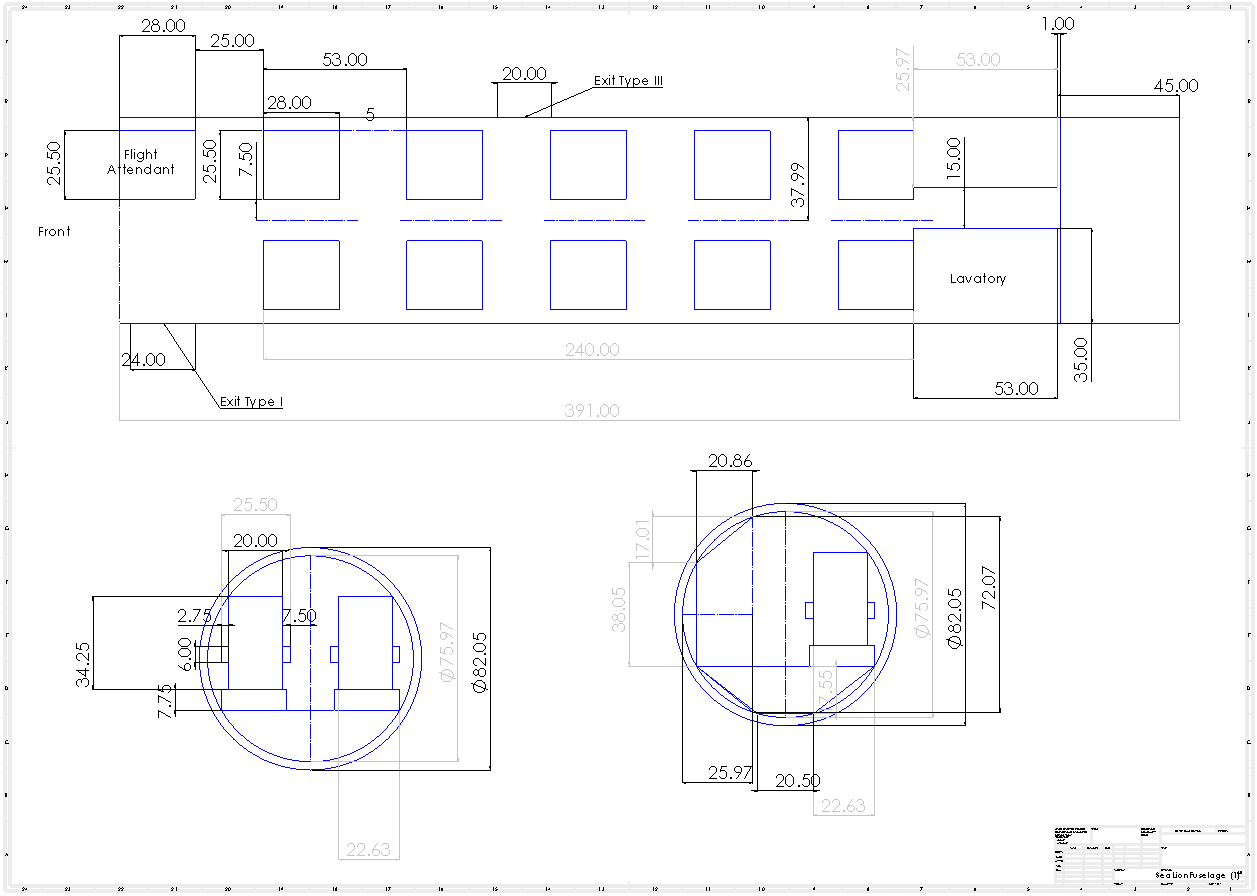
\includegraphics[angle=90, width=0.9\textwidth]{plots/fuselage_annotated}
    \caption{Fuselage layout with measurements}
    \label{fig:fuselage_annotated}
\end{figure}


\subsection{Cockpit Layout Design}
% You should include well-dimensioned cockpit layout drawings (distance from seat pan to pilot's eyes, distance from yoke to pilot, yoke travel, distance from rudder pedals to pilot and rudder travel) in this section (top and side views), including distance of pilot's eyes from the windshield, the upward and downward cockpit visibility , and the lateral cockpit visibility. Again, discuss layout decisions.

% The Twin Sea Lion is designed for a cruise $L/D$ ratio of 13. With a predicted cruise weight of 33,699 lbs, total drag force will be 2,592 lbs. 
Cockpit design was modeled on existing aircraft with similar layouts, primarily the 1930s Lockheed Electra. The design is tightly integrated around the pilot, and he sits close to the windshield, with eyes only 22 inches away. Seat dimensions and control locations were based on presentation 13 \cite{pres13} in class, which prescribes dimensions such as seat pan angle, rudder dimensions and deflections, and yoke travel requirements for a standard aircraft. The close position of the pilot was deemed necessary in order to accommodate the required vertical and horizontal fields of view in the available space for windows in the front of the Twin Sea Lion. 

Controls are standard, with a yoke from the panel and conventional rudders and throttle placement between the pilots. The two pilot's seats are side by side. No accommodations are made for a flight engineer because modern avionics and engine controls negate the need for one.

An annotated cockpit layout can be seen below in figure \ref{fig:cockpit_annotated} and an unannotated version can be seen in figure \ref{fig:cockpit} on page \pageref{fig:cockpit}.

\begin{figure}[H]
    \centering
    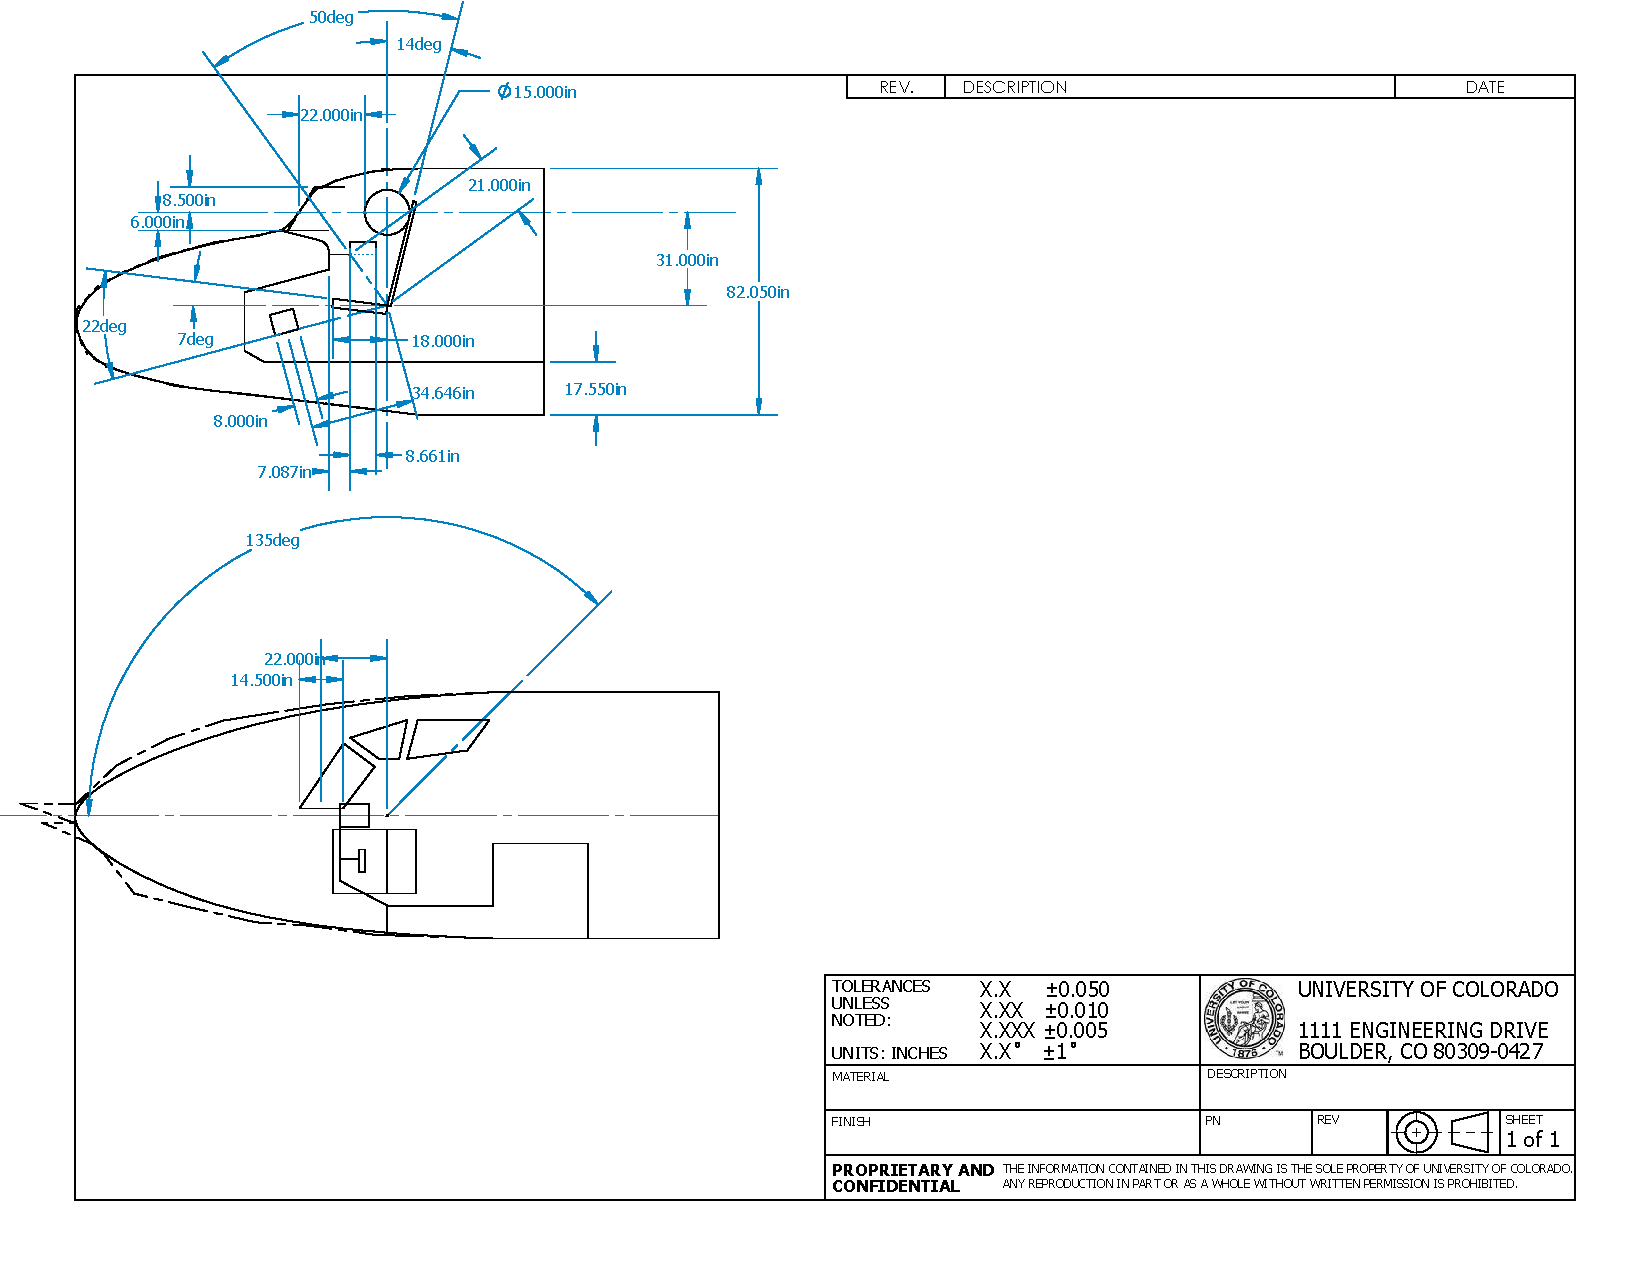
\includegraphics[angle=90, width=\textwidth]{plots/cockpit_annotated}
    \caption{Cockpit layout with measurements}
    \label{fig:cockpit_annotated}
\end{figure}

% 5
\section{Wing Layout Design}
\subsection{Airfoil Selection}
% state which airfoil was selected, along with its (t/c)max
Airfoil selection principally concerned finding an airfoil with the highest reasonable 
$C_{L_{max}}$ and the lowest possible cruise drag. The airfoils considered are tabulated in 
table \ref{tab:AirfoilOptions} on page \pageref{tab:AirfoilOptions}. The NACA 65(1)-412 airfoil was selected because 
it gives the highest lift of any airfoil found, low drag, and modest thickness at 12\%. It also features a 'drag bucket', shown in figure \ref{fig:NACA_65412B} on page \pageref{fig:NACA_65412B}, which predictions show will align with the $C_L$ required at cruise.

% check clmax of the airfoil against the needed clean CLmax of the airplane and the needed Clcruise of the airplane

% Check that CLcruise of the airplane falls in the lower part of the airfoil's drag bucket
Using a predicted cruise altitude of 30,000 feet and a speed of 350 KTAS, equation \ref{eq:q_bar} 
gives $\bar{q} = 155.4$ $lbf/ft^2$. With $S_w$, the wing area from AAA as $837 ft^2$, 
equation \ref{eq:CL} gives a predicted cruise $C_L = 0.259$ for the entire wing. Looking again at 
figure \ref{fig:NACA_65412B}, this does indeed fall in the airfoil 'drag bucket' where $C_d = 0.004$, 
and should provide good cruise performance.

% check value of cm
Again from figure \ref{fig:NACA_65412B}, $C_m$ stays nearly constant, as is desirable, at -0.8 for this airfoil.

% With cruise L/D of 13 and a cruise weight of 33698.95 lbs, the total expected drag force is 2592.2 lbs. Using standard atmosphere for 30,000 ft, this gives a whole wing where $C_L = 0.259$ and from chart \ref{fig:NACA_65412B}, $C_D = 0.004$ at this $C_L$. Roughly 520 lbs of the total drag are created by the wing here, while the other 2072 lbs come from all the other sources of drag.

% The Twin Sea Lion is deisgned for a cruise $L/D$ ratio of 13. With a predicted cruise weight of 33,699 lbs, total drag force will be 2,592 lbs. 


% http://airfoiltools.com/airfoil/details?airfoil=sc20614-il
% http://airfoiltools.com/airfoil/details?airfoil=sc20714-il#polars
% 10/16 at 5,000,000 Re as it was closest with data for 20,000,000 Re

\subsection{Geometric Design}
%You should include a wing planform drawing in this section and briefly summarize your geometric results and verify your maximum clean wing lift coefficient as discussed below

% Must have values for the following geometric design variable in this section:
% Area, Sw
% Span, bw and aspect ratio ARw
% Mean geometric chord, cw
% Taper ratio \lambda w
% Quarter-chord sweep angle \Lambda c/4w
% Dihedral, \Gamma w
% Incidence angle, i w
% wing twist angle \epsilon w

Since the wing is a straight tapered planform, the mean geometric chord can be calculated as follows.

\begin{equation}
    \bar{c}_w = c_r \frac{1 + \lambda}{2}
\end{equation}

With $c_r$ selected as 12.7 feet and $\lambda_W = 0.6$, $\bar{c}_W = 10.16$ feet.

Incidence angle was based on where the plain airfoil reaches the appropriate lift coefficient for cruise as calculated below.

\begin{equation}
    W_C = W_{TO} - 0.4 W_F
\end{equation}
\begin{equation}
    C_L = \frac{ W_C }{ \bar{q} S}
\end{equation}

In cruise conditions, $C_L = 0.259$, which is actually below the zero-lift angle of attack of 0.35, so it was decided to mount the wings at a $-1.5 ^\circ$ angle of incidence so that the aircraft will cruise with the nose perfectly level. The airfoil still stays in the regime of minimum drag at this angle of attack.

As an alternative, the designers considered twisting the wingtips downwards to improve roll control during stall and reduce cruise $C_L$. However, this line of inquiry was dropped on the basis of geometric complexity and lack of access to the advanced aerodynamic modeling needed to determine the appropriate amount and distribution of twist needed to achieve these goals.

From Table 6.6 in \cite{WingGeometryGerren} and tabulated in table \ref{tab:SelectedWingGeometry} in the appendix, most regional airliners have no wing twist, solidifying the decision to keep the wingtips level. In addition, this data was used to make and educated guess at the appropriate dihedral angle $\Gamma_W$. The average dihedral angle of the selected aircraft is $4.67 ^\circ$. Thus, $\Gamma_W = 5^\circ$ was selected as a reasonable value but if anything, this may have to be increased in the future to accommodate the anticipated ground clearance requirements of the propellers and the destabilizing effects of the low mounted wing. Most of the low wing aircraft in the aforementioned table have dihedral angles of $7^\circ$.

The final geometric design variables are tabulated below in table \ref{tab:SelectedWingGeometry} and shown graphically in figure \ref{fig:StraightTaperedWingGeometryPlot}.

\begin{table}[H]
\centering
\caption{Geometric design variables}
\label{tab:WingGeometry}
\begin{tabular}{|c|c|c|c|c|c|c|c|c|} \hline
$S_W$ [$ft^2$] & $b_w$ [ft] & $AR_W$ & $c_w$[ft] & $\lambda_W$ & $\Lambda_{c/4w}$[$^\circ$] & $\Gamma_W$[$^\circ$]  & $i_W$[$^\circ$] & $\epsilon_W$[$^\circ$]\\ \hline
837 & 81.8 & 8 & 10.16 & 0.6 & 0 & 5 & -1 & 0\\ \hline
\end{tabular}
\end{table}

\begin{figure}[H]
	\centering
	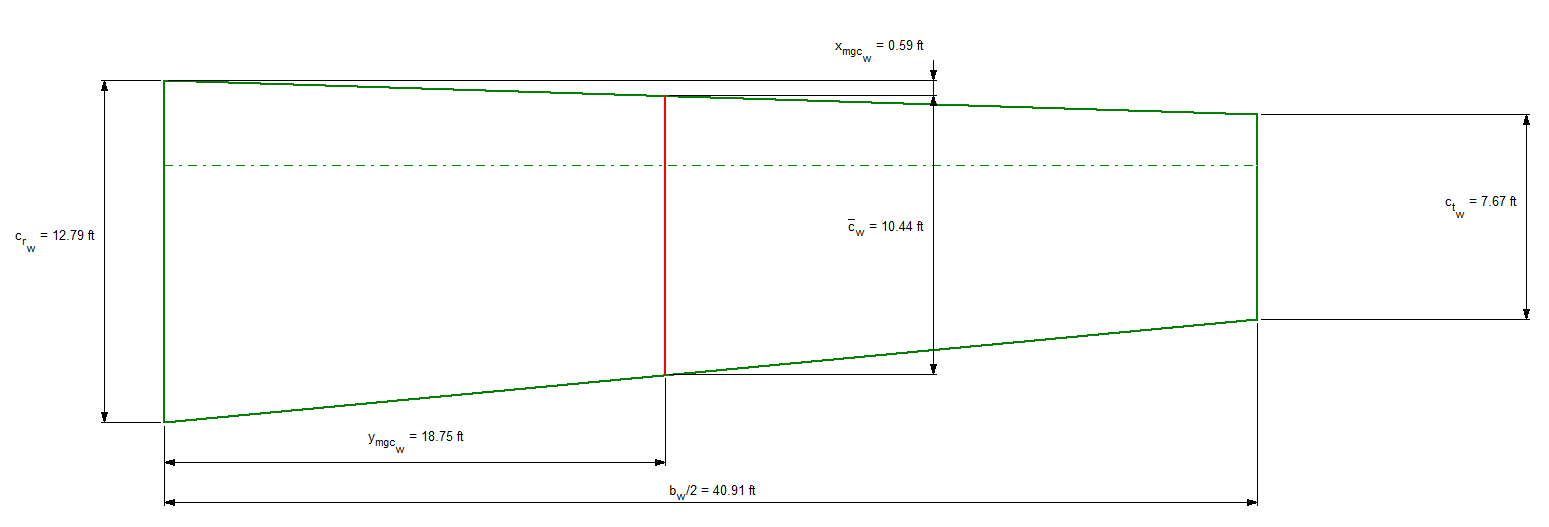
\includegraphics[width=\textwidth]{TwinSeaLionReport2Printouts/StraightTaperedWingGeometryPlot}
	\caption{Straight tapered wing geometry plot}
	\label{fig:StraightTaperedWingGeometryPlot}
\end{figure}

\subsection{Critical Mach Number Check}
% you should perform a critical Mach number check, if applicable. Mcr plots are found in class handouts and in Canvas. Show where you point lies on the critical Mach number plot
Based on the graph in figure \ref{fig:Mcr_check} on page \pageref{fig:Mcr_check}, the critical Mach number of the chosen NACA 65(1)-412 airfoil is $M=0.75$, well above the intended cruise speed of the Twin Sea Lion. Our design point is circled at the very bottom left corner of the graph. No shocks are expected on the upper surface of the wing.

\subsection{Fuel Volume of Wing}
% you need to calculate fuel volume available in wing and state whether it is sufficient or not. If not, state available places being considered for storage of rest of fuel
The surface is substantial, and AAA indicated a healthy margin for fuel as shown in figure \ref{fig:WingFuelVolume}. The Twin Sea Lion requires 10,679 pounds to achieve its 1500 nautical mile range and the wings have room for 20,559 pounds. Combined with more efficient than expected engines, no fuel issues are expected. Data from AAA can be seen in figure \ref{fig:WingFuelVolume}.

% 6
\section{Layout Design of the High Lift Devices}
\subsection{Sizing the High Lift Devices}
%You should include a wing planform drawing in this section with leading and trailing edge high lift devices drawn in. Discuss design decisions which led to selection of high lift devices used
The flap planform layout can be found in figure \ref{fig:HighLiftDeviceSizingPlot} below. Single slotted flaps were chosen for the Twin Sea Lion as they were found to fit the takeoff and landing performance requirements. Takeoff turned out to be the constraining limitation, at $20^\circ$ deflection, the flaps needed to be 30\% of the wing chord and span from 9\% to 55.5\% of the wing in order to achieve the improvement in $C_L$ needed. Landing with a flap deflection of $30^\circ$ was not a constraining factor. This makes intuitive sense with the adage that, "an airplane can land somewhere it can't take off from," referring to ground roll and obstacle clearance requirements. These numerical results can be seen in figure \ref{fig:HighLiftDeviceSizing} on page \pageref{fig:HighLiftDeviceSizing}.

Ailerons were sized to fit the remaining span of each wing, going from 60\% to 98\% of the half span, and taking up 25\% of the wing chord.

\begin{figure}[H]
	\centering
	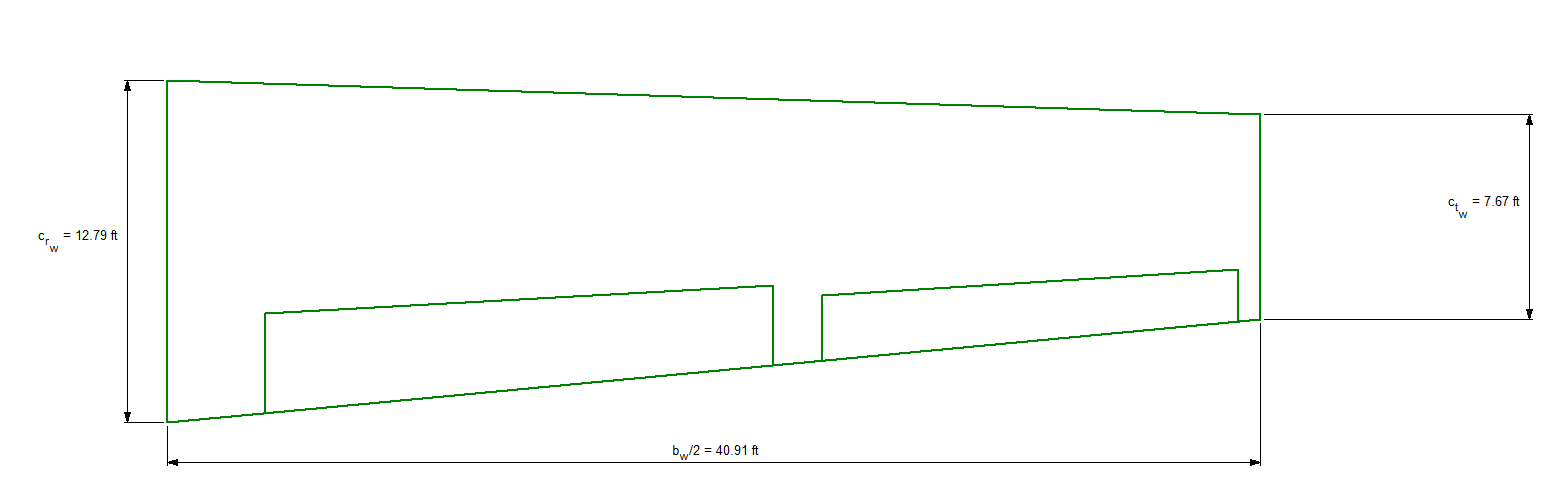
\includegraphics[width=\textwidth]{TwinSeaLionReport2Printouts/HighLiftDeviceSizingPlot}
	\caption{High lift device sizing plot}
	\label{fig:HighLiftDeviceSizingPlot}
\end{figure}

\subsection{Verifying the High Lift Devices}
%verify that your high lift devices give you the C. needed for takeoff and landing and briefly summarize your results. What flap deflections are needed to achieve you takeoff and landing Cl values?
AAA gives an improvement in takeoff $C_L$ of $\Delta C_{L_{w_{TO}}} = 0.4715$, for a takeoff $C_{L_{max}} = 2.1215$, beating the requirement of $C_{L_{TO}} = 2.1$. Landing $C_L$ was designed to be 2.2. With $\Delta C_{L_{w_{L}}} = 0.5765$, for $C_{L_{max}} = 2.1965$, which felt close enough to the predicted landing requirements given the lack of landing constraints. Should this prove to become a limiting factor in the future, plenty of room remains to enlarge the flaps, add more slots, or include leading edge devices such as slats and vortex generators.

\section{Selection and Integration of the Propulsion System}
\subsection{Selection of the Propulsion System}
% Explain what engine was selected for your aircraft and why. Does it meet you cj or cp requirements? does it operate for your altitude and speed needed
The engine was chosen in order to supply the high horsepower needed by the aircraft. The Sea Lion also needs a low $c_p$ in order to maintain current weights. The Pratt and Whittney PW150A turboprop engine was chosen for its high power and very good efficiency. The PW150A can produce up to 5000 SHP and has a $c_p$ of $0.433 lbs/hp \times hr$. This well exceeds our maximum power requirement of TBD and this engine's most common application, the Q-400, cruises only 5,000 feet lower at similar speeds. \cite{PW150FuelFlow}
Because the initially planned engine performance included a $c_p$ of 0.6, the improved efficiency gives a comfortable margin over our intended range and provides improved capabilities.

\subsection{Integration of the Propulsion System}
% Explain where you are installing the engines for your aircraft and why, including engine 
% dimensions. Can it physically fit in/on the aircraft? What are the advantages or disadvantaes of this installation?
The engines will be installed on the wings. Since this aircraft required multiple engines, placing 
them here provides symmetry. Additionally, the engine must be placed away from the fuselage by 
at least the radius of the propeller. The chosen Pratt and Whittney PW150A engine is 7.9 feet long, 
which fits onto our wing structure. However, propeller diameters will likely be quite large and necessitate mounting the engines above the wing slightly. Because the Sea Lion uses turboprops rather than turbojets, the presence of the engines will not reduce available flap area. The prop wash over the wing may, in fact, slightly increase the available lift.

\subsection{Installed Thrust}
%calculate installed thrust (this is usable thrust - it is not the thrust given by the engine manufactures. Does it meet your Tto requirements
A variety of accessories need to be run off engine power, including electrical, pneumatic, and hydraulic, systems. These all reduce the flying power available. Figures \ref{fig:engineelecpowerextraction} through \ref{fig:engineTotalPowerExtraction} in the appendix show the calculations. Mechanical systems, including all the pumps, take a total of 10.07 horsepower from each engine. Electrical systems extract 4 horsepower, and pneumatic systems 75 horsepower. After all the accessories are accounted for, the engines still transmit 4715 horsepower to the driveshaft. 

The driveshaft connects to the gearbox and propeller, which each introduce their own losses. The gearbox is assumed to be 98\% efficient and the propeller is 90\% efficient. These reduce the effective power to 4,243 horsepower per engine, or 8,486 total horsepower. This remains well above the power requirements.

\section{Conclusions and Recommendations}
\subsection{Conclusions}
In summary, the Twin Sea Lion has begun to take shape for its mission. Despite the need to reduce planned cruising speed, initial results show that this aircraft can fit its mission requirements with room to spare. Passengers will have De Luxe sized seats, sitting one on each side of the aisle and five rows deep. While cargo storage solutions were forced to become innovative, everything required was fit into a compact fuselage and room for a lavatory was found. The selection of a low-wing will improve the stiffness of future landing gear. A NACA 65(1)-412 airfoil shows promise and modest flaps fit all takeoff and landing requirements. The overall wing design lacks complications such as twisted or curved leading and trailing edges. The wing also includes ample room for fuel. Coupled with highly efficient PW150A engines, range is no issue, even accounting for power lost to accessory drives. However, propeller choices will have to be made carefully in order to ensure continued high efficiency.

\subsection{Recommendations}
Future work for the Twin Sea Lion designers will delve into exact configurations and equipment balance. However, it may prove beneficial to review power and wing loading requirements. Current power loading is 4.4 pounds per horsepower. Based on the revised performance sizing chart shown in figure \ref{fig:new_perf_sizing}, this may afford a smaller wing - possibly even double the current wing loading. Currently, the constraining requirement on wing size is takeoff performance. A smaller wing, coupled with more aggressive flaps could result in higher cruise speed and better economy.

% 7
%\renewcommand{\refname}{\section{Sources}}
%\section{References}
\begin{thebibliography}{99}
% Twin Otter: https://www.vikingair.com/sites/default/files/documents/Twin%20Otter%20Series%20400%20Multi-Page%20Brochure.pdf
\bibitem{dhc-6} Twin Otter Series 400. Viking Air, 
    \url{https://www.vikingair.com/sites/default/files/documents/Twin Otter Series 400 Multi-Page Brochure.pdf}

% PC-24: https://www.pilatus-aircraft.com/en/fly/pc-24 | Weight from Wikipedia
% https://www.pilatus-aircraft.com/data/document/Pilatus-Aircraft-Ltd-PC-24-Factsheet.pdf
\bibitem{pc24Wto} PC-24 The Super Versatile Jet. Pilatus, 
        \url{http://www.pilatus-aircraft.com/data/document/Pilatus-Aircraft-Ltd-PC-24-Factsheet.pdf}
%empty weight: https://www.militaryfactory.com/aircraft/detail.asp?aircraft_id=1256#specs
\bibitem{pc24We} "Pilatus PC-24 Light Passenger Jet Aircraft - Switzerland." Military Weapons, 
    \url{http://www.militaryfactory.com/aircraft/detail.asp?aircraft_id=1256#specs}

% DHC-4: http://www.dhc4and5.org/caribou_manuals.htm
\bibitem{dhc-4} "C-7A Flight Manual Performance Data." Wayne E. Buser, 
    \url{http://www.dhc4and5.org/caribou_manuals.htm}

% F-27: https://www.planeandpilotmag.com/article/fairchild-hiller-fh-227-fokker/
\bibitem{F-27} "FAIRCHILD HILLER FH-227 (FOKKER)" Plane and Pilot Magazine, 
    \url{https://www.planeandpilotmag.com/article/fairchild-hiller-fh-227-fokker/}

% Q-400: https://www.airliners.net/aircraft-data/de-havilland-canada-dhc-8-400-dash-8/122
\bibitem{Q400} "De Havilland Canada DHC-8-400 Dash 8." Airliners.net, 
    \url{http://www.airliners.net/aircraft-data/de-havilland-canada-dhc-8-400-dash-8/122}

% http://www.flugzeuginfo.net/acdata_php/acdata_f27_en.php
\bibitem{F-27-length} "Fokker F27 Friendship" Flugzeuginfo Info,
    \url{http://www.flugzeuginfo.net/acdata_php/acdata_f27_en.php}

% https://www.pprune.org/tech-log/353486-q400-fuel-burn.html#post4583597
\bibitem{PW150FuelFlow} "Q-400 Fuel Burn?" Professional Pilot's Rumor Network,
    \url{https://www.pprune.org/tech-log/353486-q400-fuel-burn.html#post4583597}

\bibitem{AirfoilBook} Abbott and Doenhoff, \textit{Theory of Wing Sections}. "Including a Summary of Airfoil Data" Dover Publications, Inc. New York, 1959.

\bibitem{MachCheckBook} Roskam, \textit{Airplane Design} "Part II: Preliminary Configuration Design and Integration of the Propulsion System". University of Kansas. Lawrence, Kansas. 1989.

\bibitem{WingGeometryGerren} Gerren, "Wing Geometry Tables", \url{https://canvas.colorado.edu}

\bibitem{pres12} Gerren, "Presentation 12", \url{https://canvas.colorado.edu}

\bibitem{pres13} Gerren, "Presentation 13", \url{https://canvas.colorado.edu}

\end{thebibliography}

% 8
\section*{Appendix}

\subsection*{Equations}
Dynamic Pressure
\begin{equation}
    \bar{q} = \frac{1}{2} \rho V^2
    \label{eq:q_bar}
\end{equation}

$C_L$ of a wing
\begin{equation}
    C_L = \frac{L}{ \bar{q} S }
    \label{eq:CL}
\end{equation}

\subsection*{Airfoil Data}
\begin{figure}[H]
    \centering
    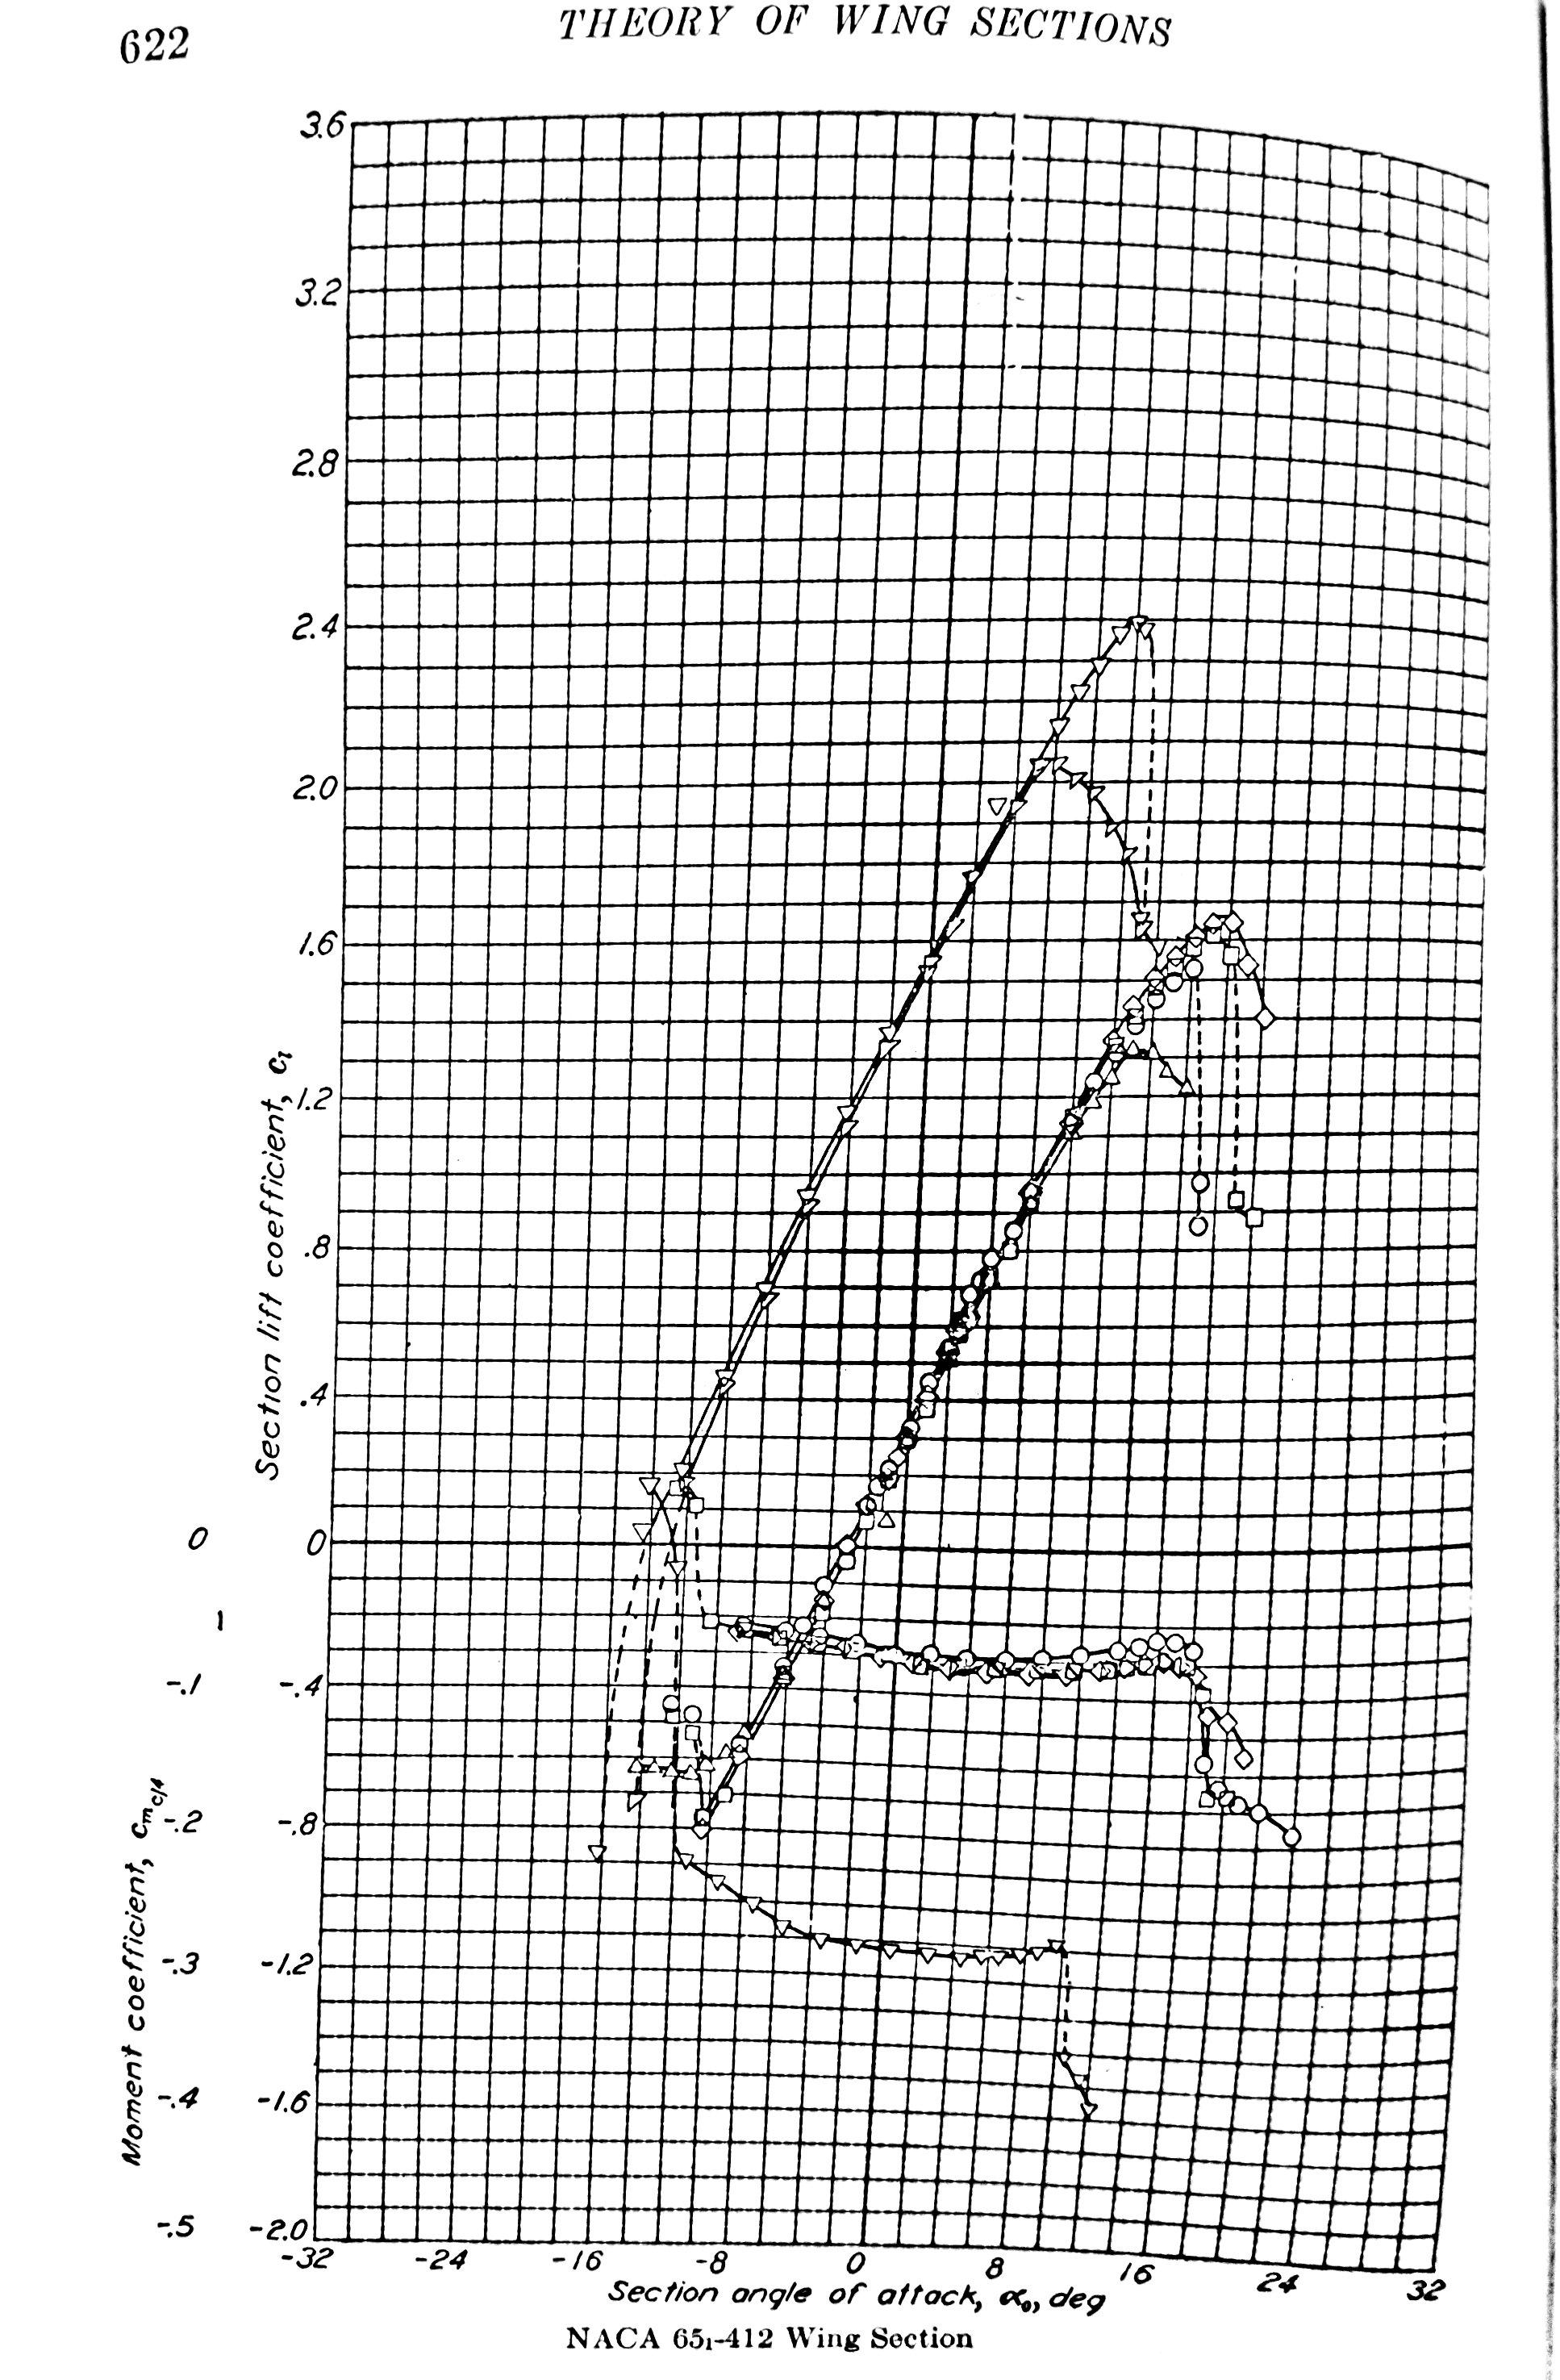
\includegraphics[width=0.7\textwidth]{plots/Airfoil65_1_412-a}
    \caption{NACA 65(1)-412 performance chart 1}
    \label{fig:NACA_65412A}
\end{figure}
\begin{figure}[H]
    \centering
    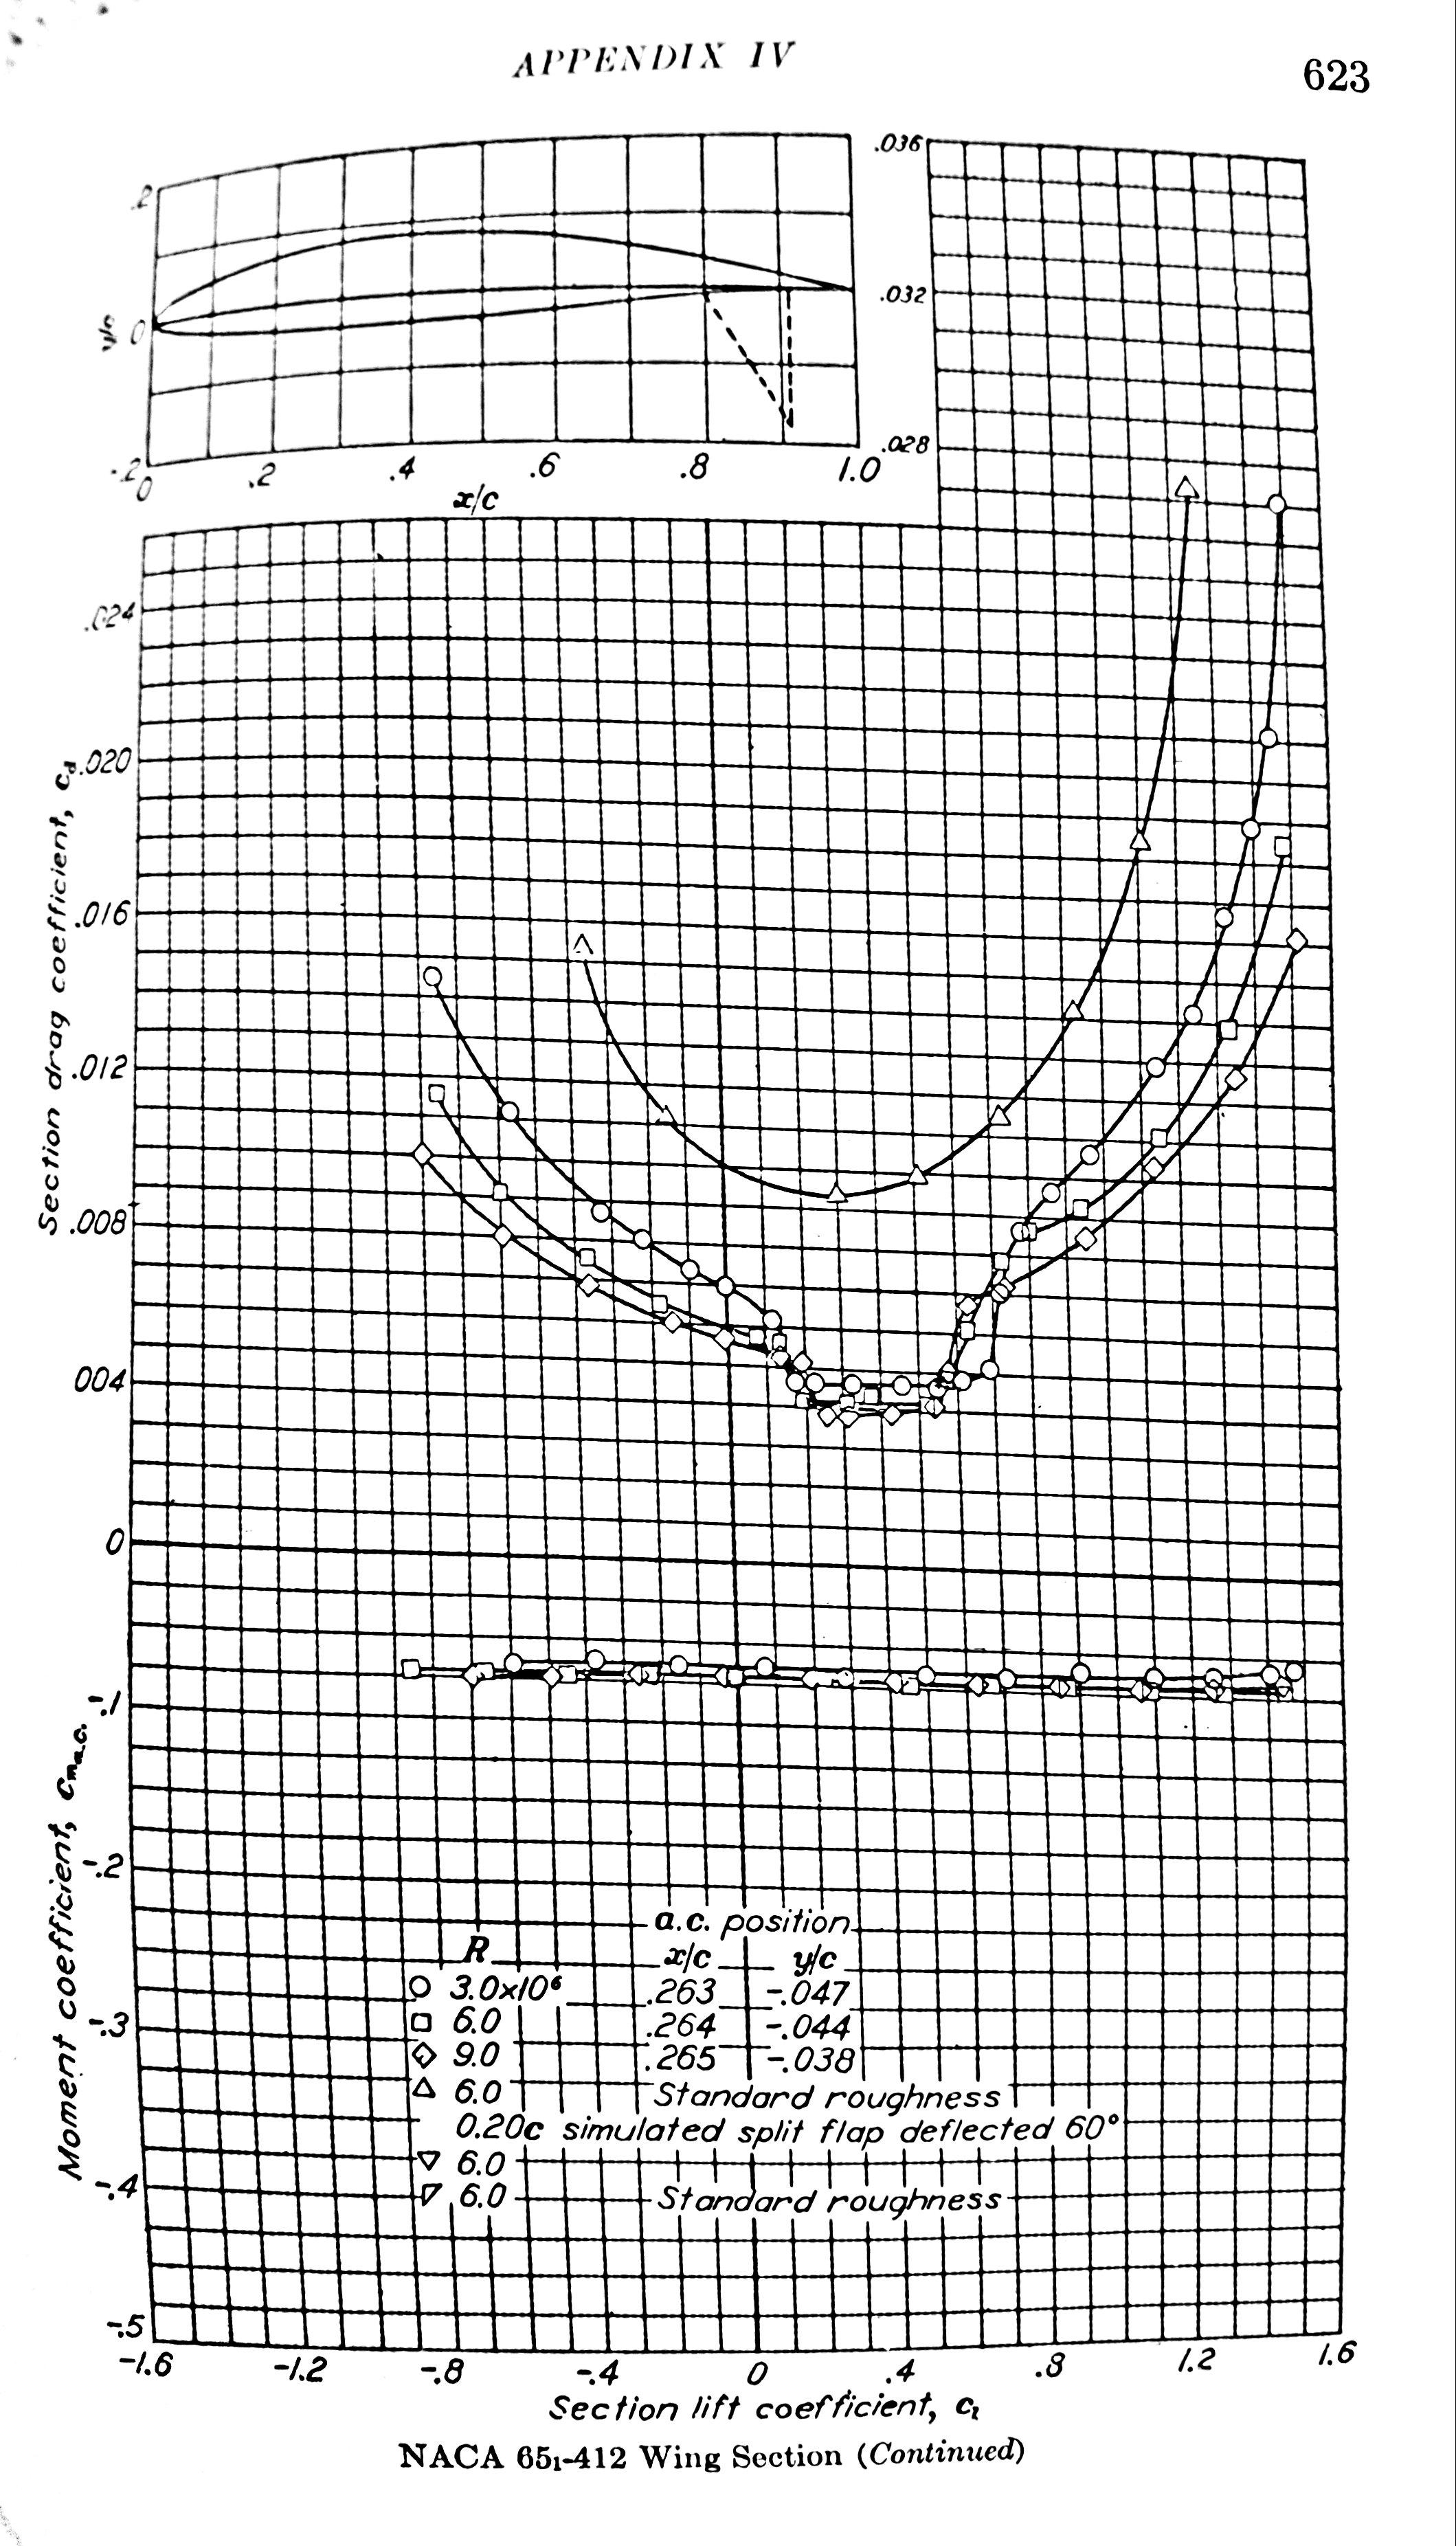
\includegraphics[width=0.7\textwidth]{plots/Airfoil65_1_412-b}
    \caption{NACA 65(1)-412 performance chart 2}
    \label{fig:NACA_65412B}
\end{figure}
\begin{figure}[H]
    \centering
    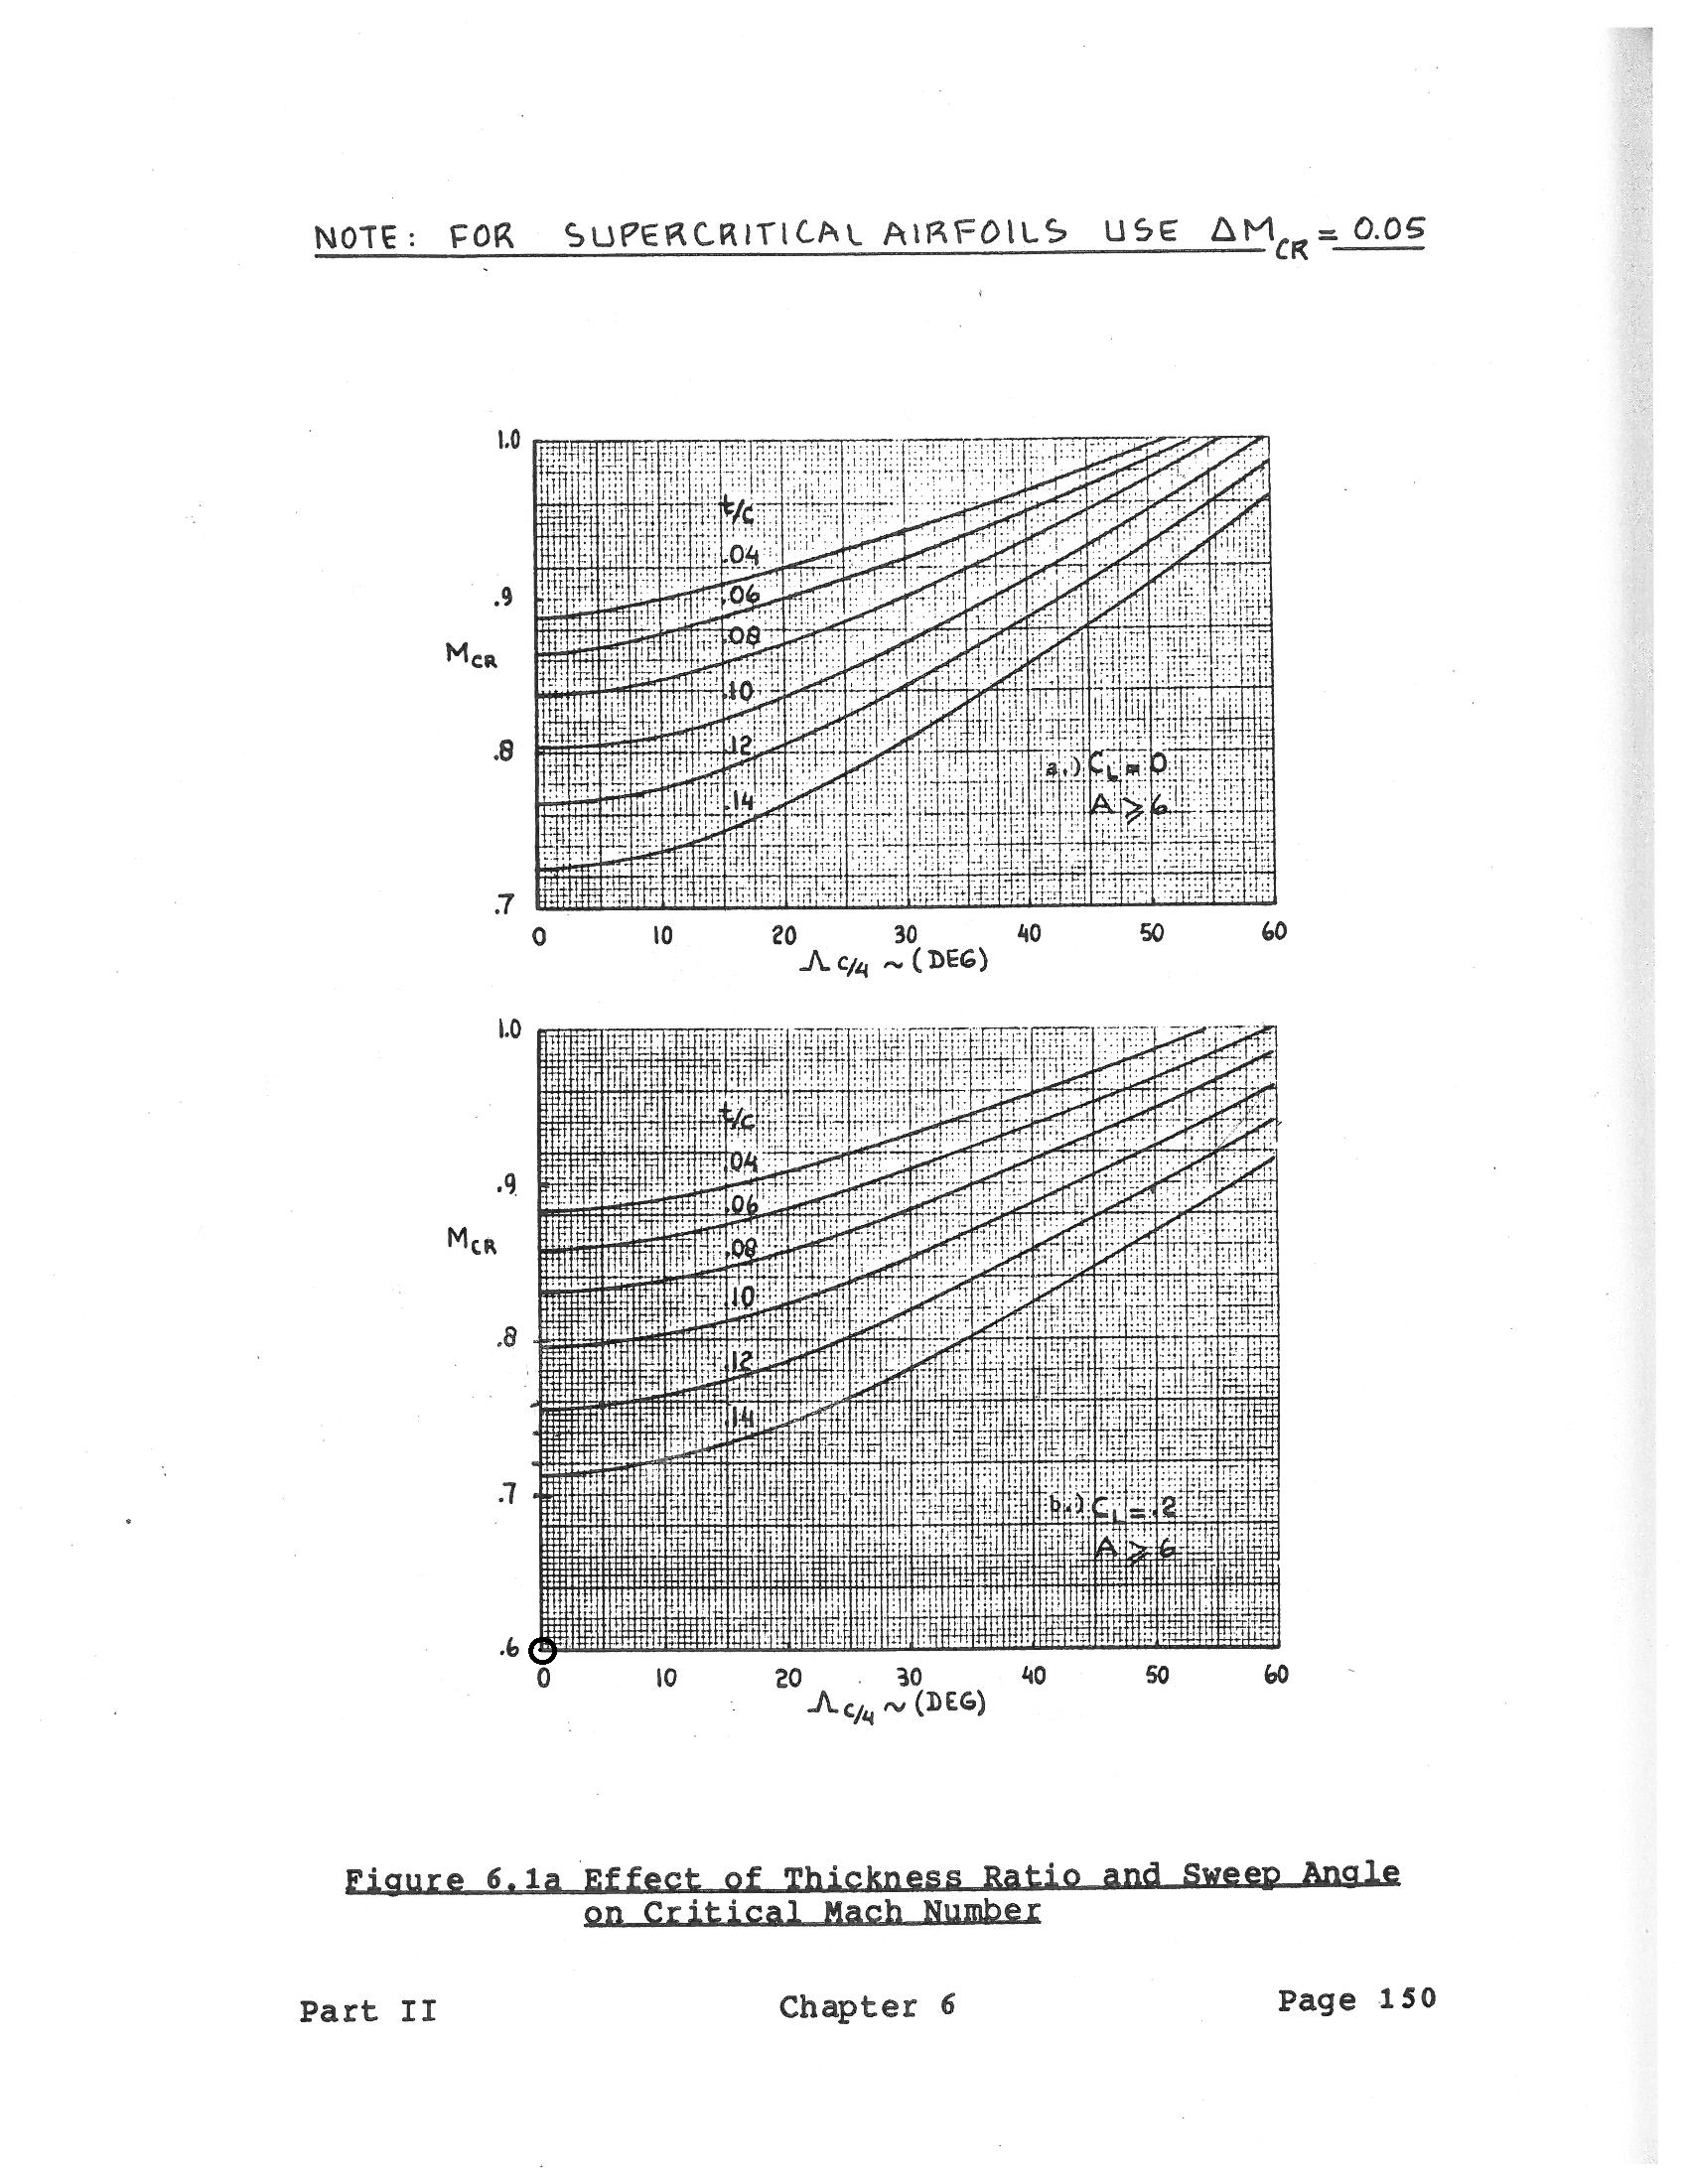
\includegraphics[width=\textwidth]{plots/Mcr_check}
    \caption{Critical mach number check}
    \label{fig:Mcr_check}
\end{figure}

\subsection*{Cockpit and Fuselage Dimensions}
\begin{figure}[H]
    \centering
    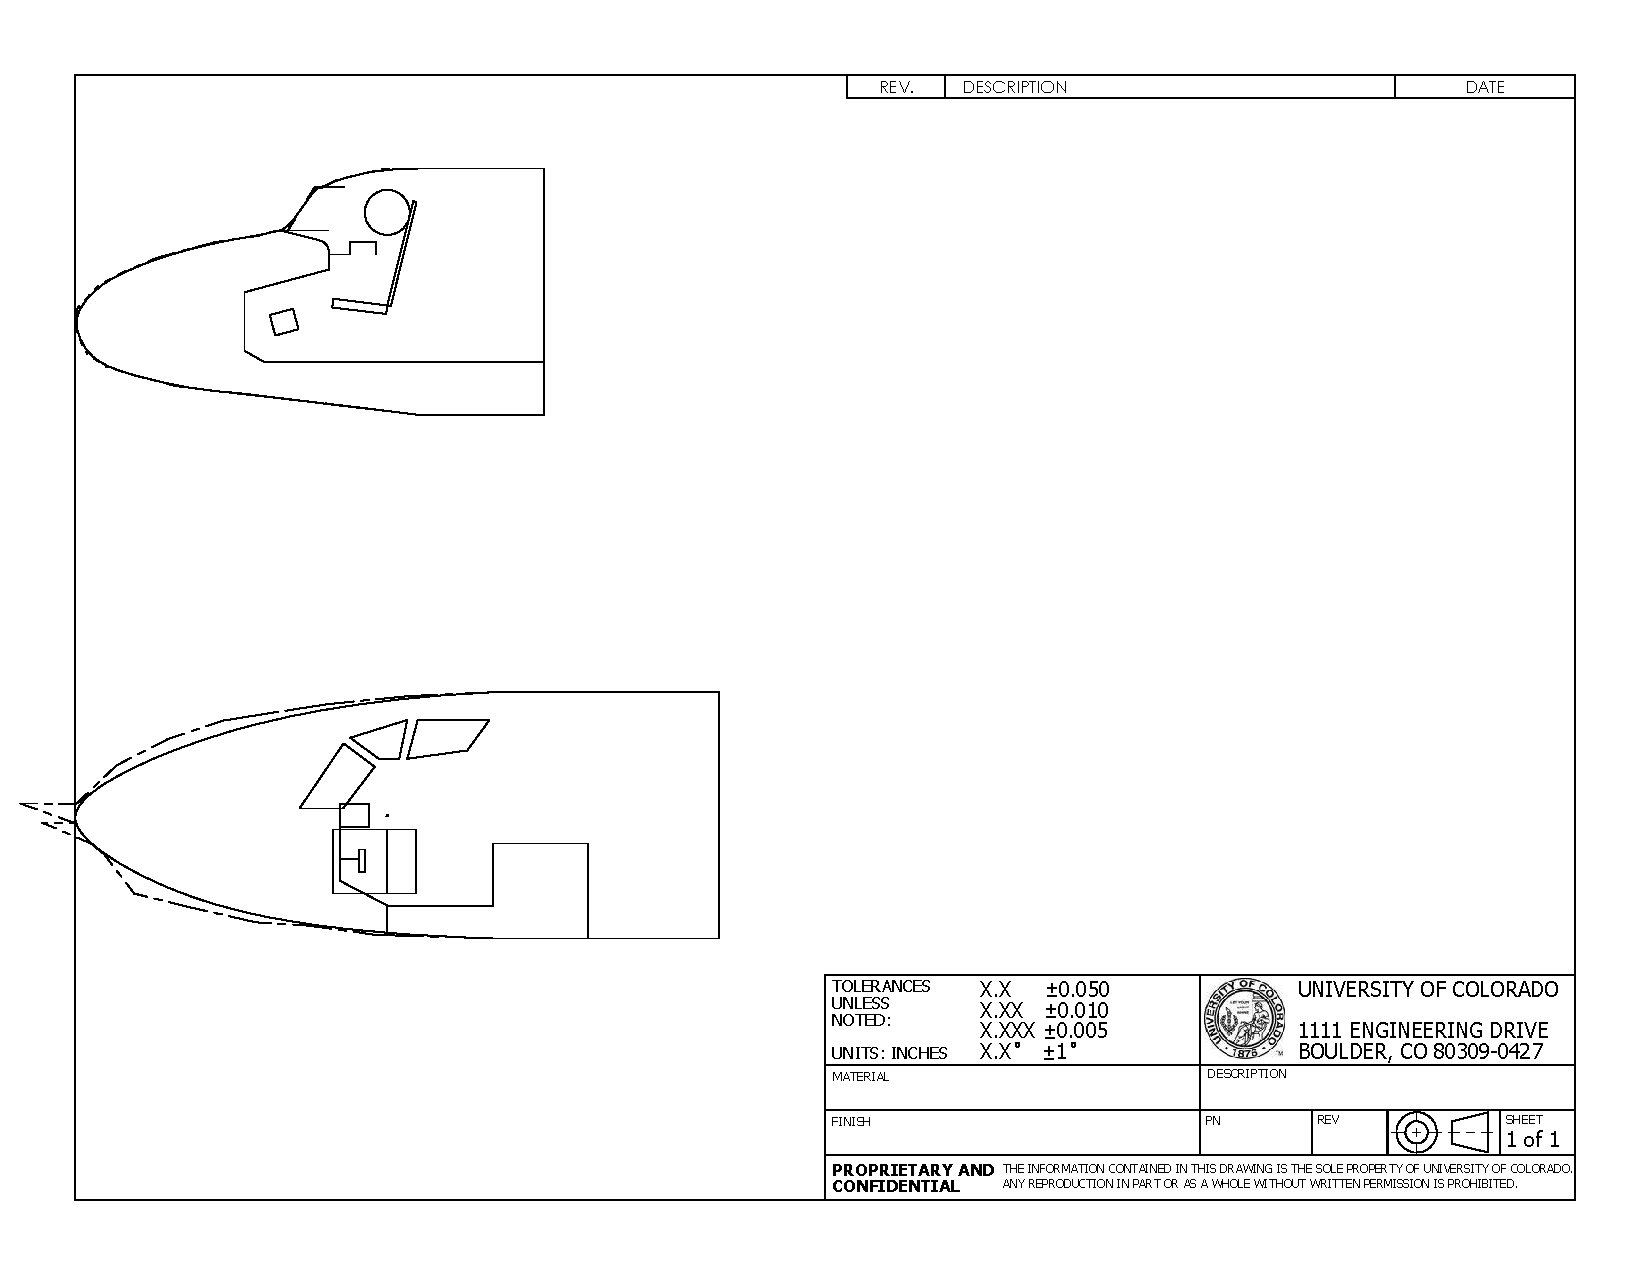
\includegraphics[angle=90, width=\textwidth]{plots/cockpit}
    \caption{Cockpit layout}
    \label{fig:cockpit}
\end{figure}
%%MOVED TO FUSELAGE SECTION
%\begin{figure}[H]
%    \centering
%    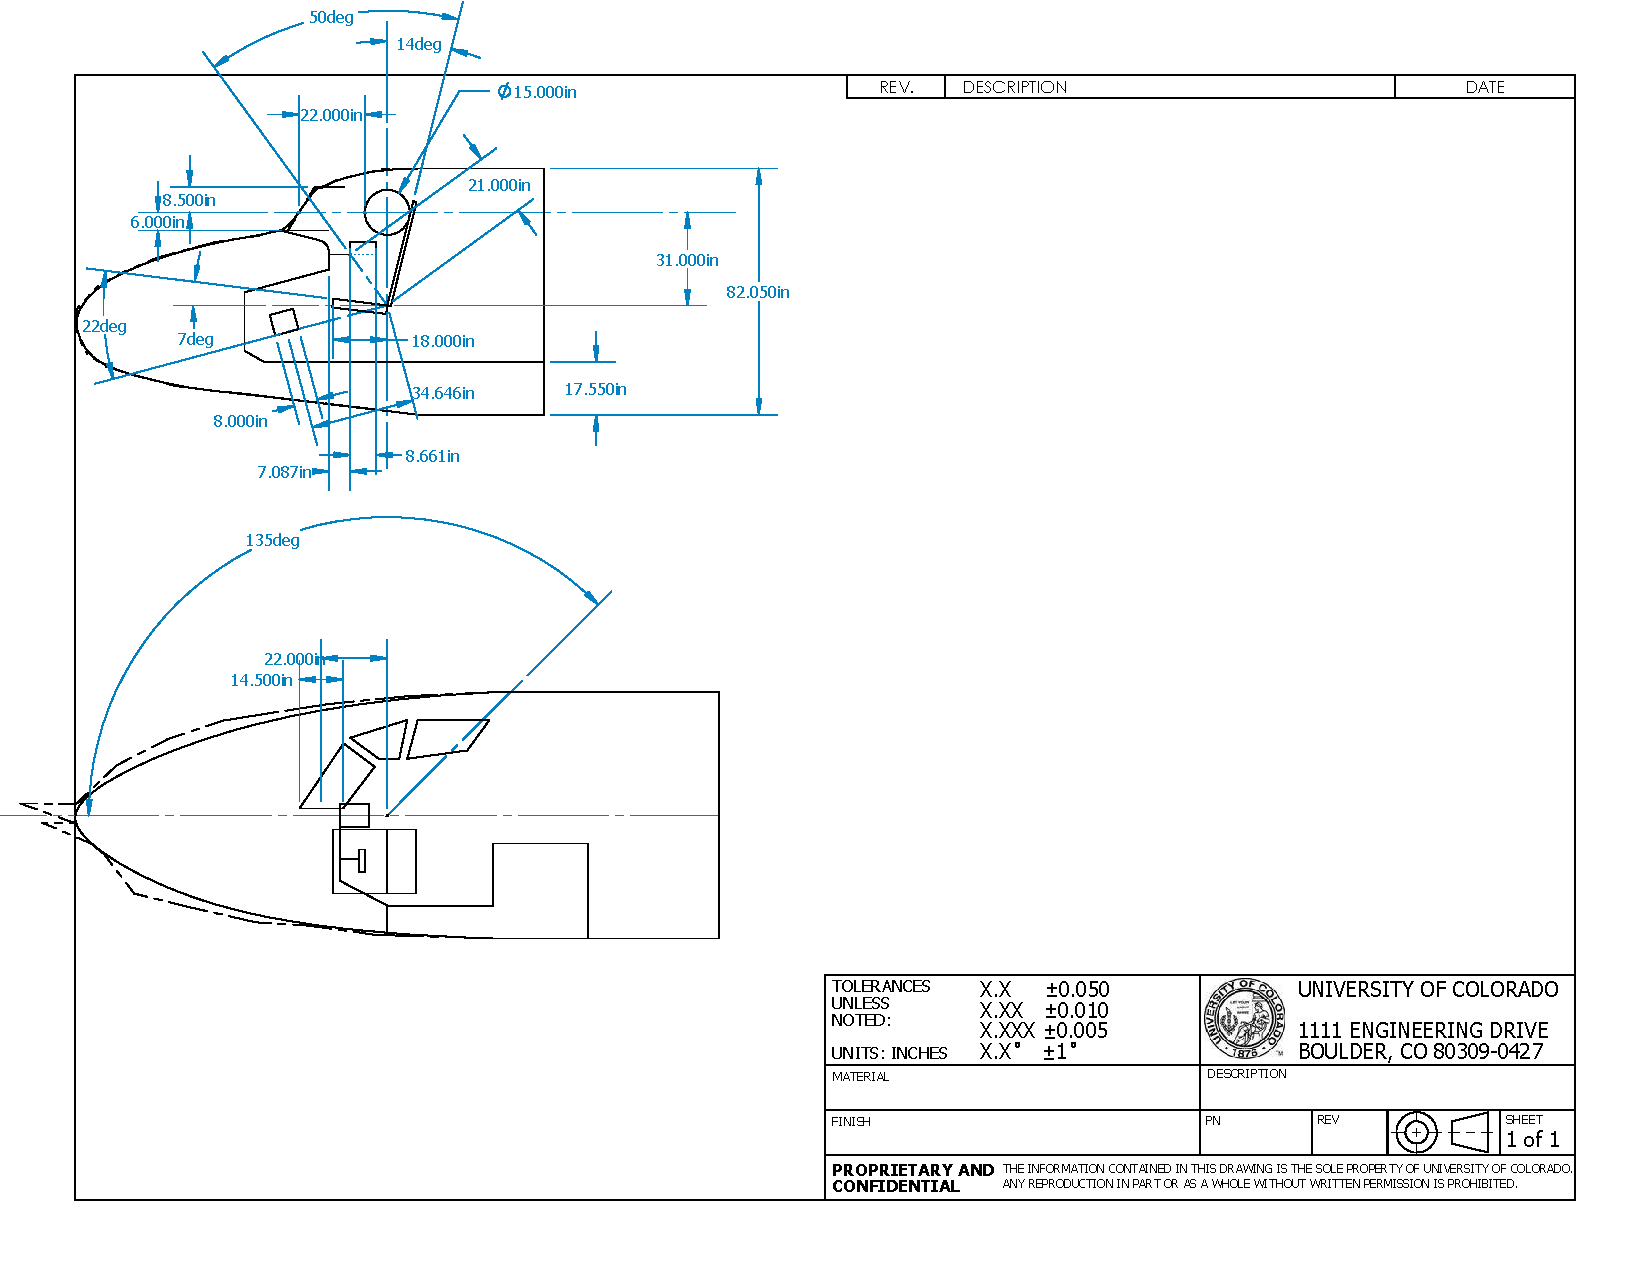
\includegraphics[angle=90, width=\textwidth]{plots/cockpit_annotated}
%    \caption{Cockpit layout with measurements}
%    \label{fig:cockpit_annotated}
%\end{figure}
%\begin{figure}[H]
%    \centering
%    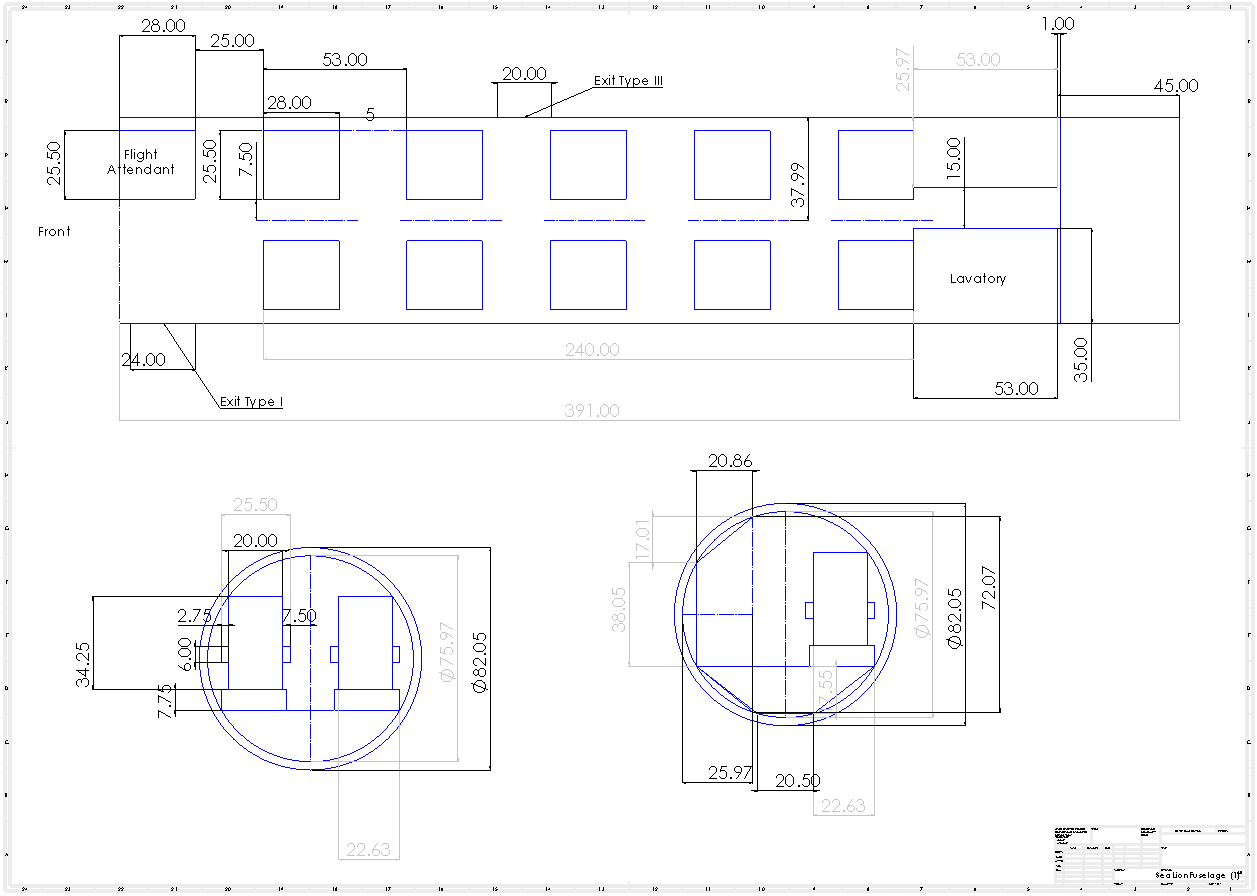
\includegraphics[angle=90, width=0.9\textwidth]{plots/fuselage_annotated}
%    \caption{Fuselage layout with measurements}
%    \label{fig:fuselage_annotated}
%\end{figure}

\subsection*{Data from AAA}
\begin{figure}[H]
	\centering
	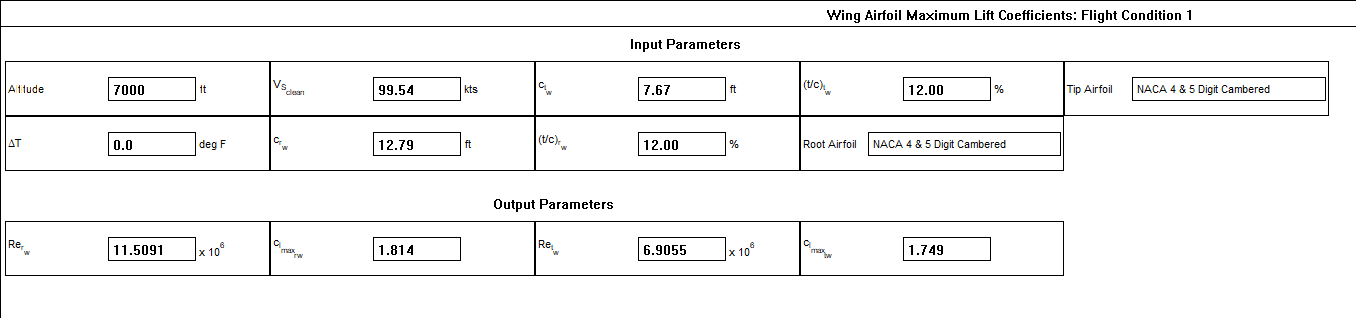
\includegraphics[width=\textwidth]{TwinSeaLionReport2Printouts/AirfoilMaximumLiftCoefficients}
	\caption{Airfoil maximum lift coefficients}
	\label{fig:AirfoilMaximumLiftCoefficients}
\end{figure}
\begin{figure}[H]
	\centering
	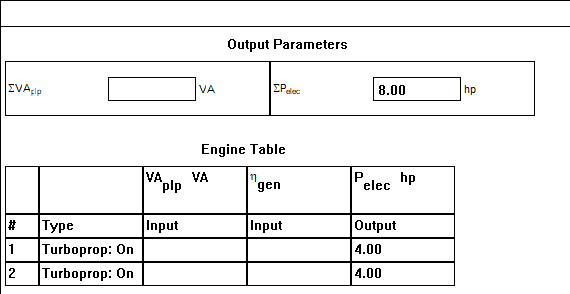
\includegraphics[width=\textwidth]{TwinSeaLionReport2Printouts/engineelecpowerextraction}
	\caption{Engine electrical power extraction}
	\label{fig:engineelecpowerextraction}
\end{figure}
\begin{figure}[H]
	\centering
	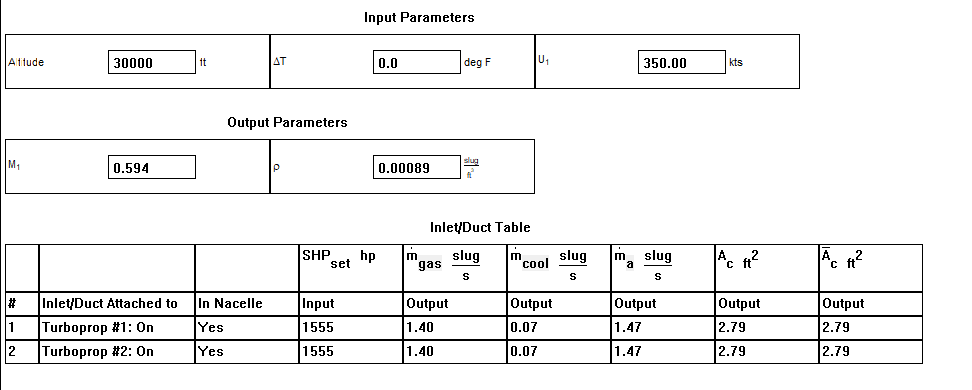
\includegraphics[width=\textwidth]{TwinSeaLionReport2Printouts/engineInletArea}
	\caption{Engine inlet area}
	\label{fig:engineInletArea}
\end{figure}
\begin{figure}[H]
	\centering
	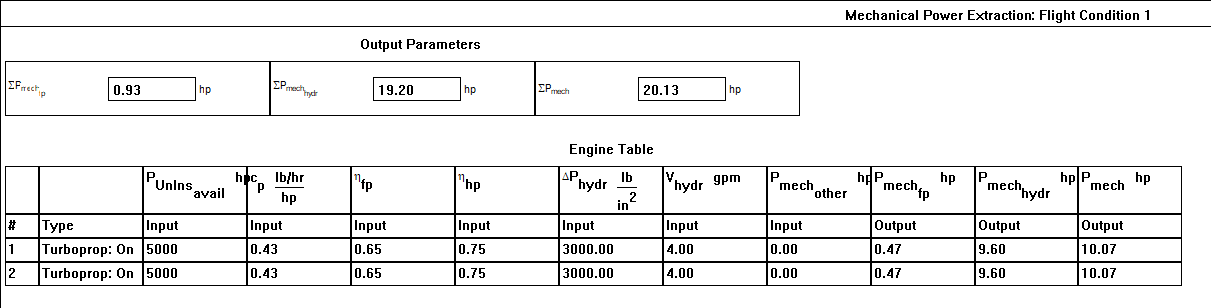
\includegraphics[width=\textwidth]{TwinSeaLionReport2Printouts/enginemechpowerextraction}
	\caption{Engine mechanical power extraction}
	\label{fig:enginemechpowerextraction}
\end{figure}
\begin{figure}[H]
	\centering
	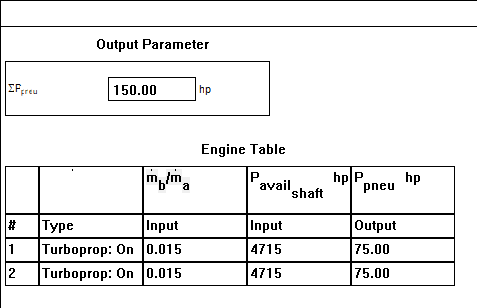
\includegraphics[width=\textwidth]{TwinSeaLionReport2Printouts/enginepneumaticpowerextraction}
	\caption{Engine pneumatic power extraction}
	\label{fig:enginepneumaticpowerextraction}
\end{figure}
\begin{figure}[H]
	\centering
	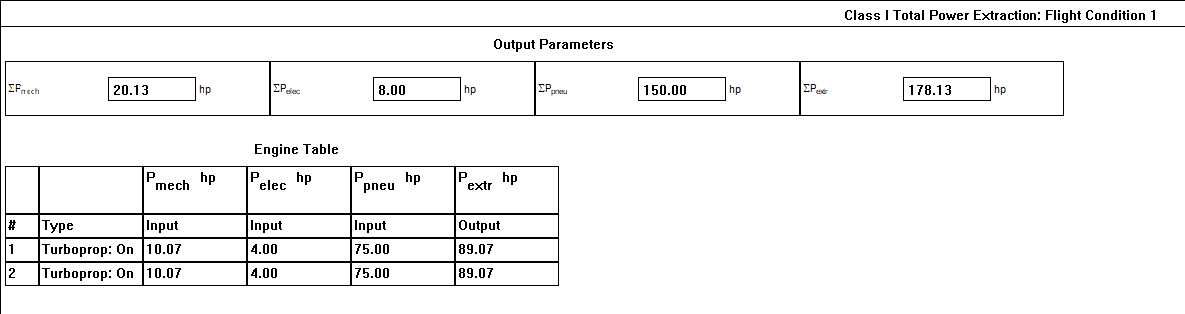
\includegraphics[width=\textwidth]{TwinSeaLionReport2Printouts/engineTotalPowerExtraction}
	\caption{Engine total power extraction}
	\label{fig:engineTotalPowerExtraction}
\end{figure}
\begin{figure}[H]
	\centering
	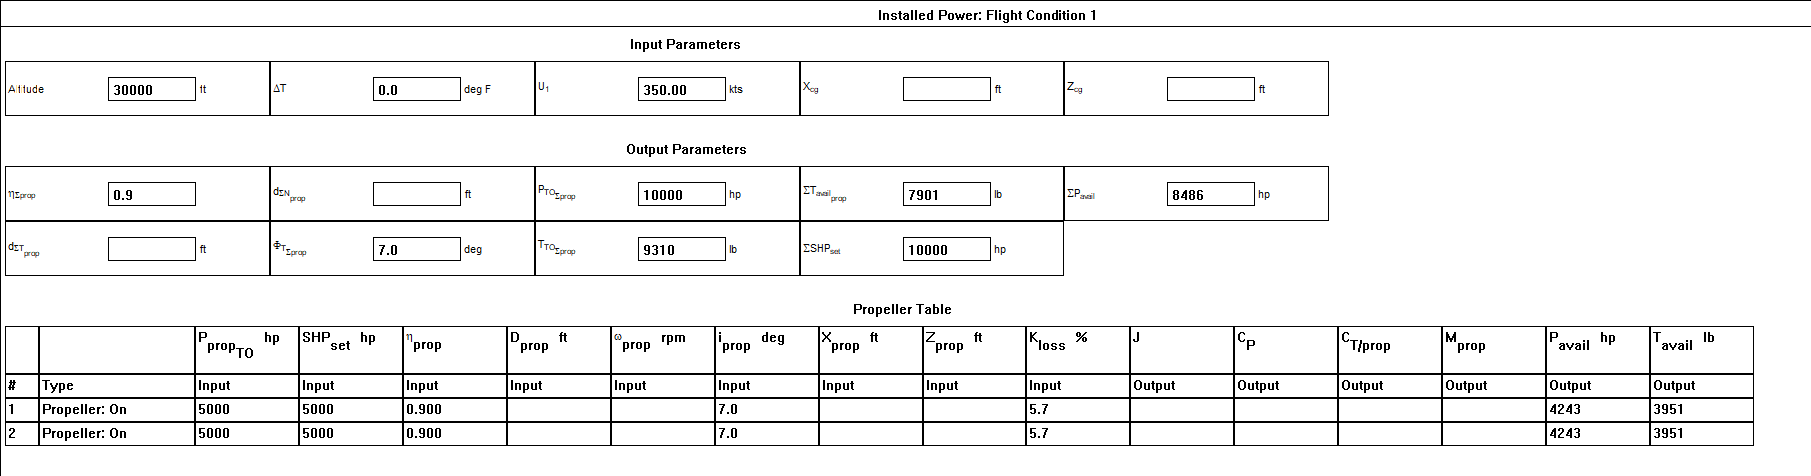
\includegraphics[width=\textwidth]{TwinSeaLionReport2Printouts/engineInstalledPower}
	\caption{Engine installed power}
	\label{fig:engineInstalledPower}
\end{figure}
\begin{figure}[H]
	\centering
	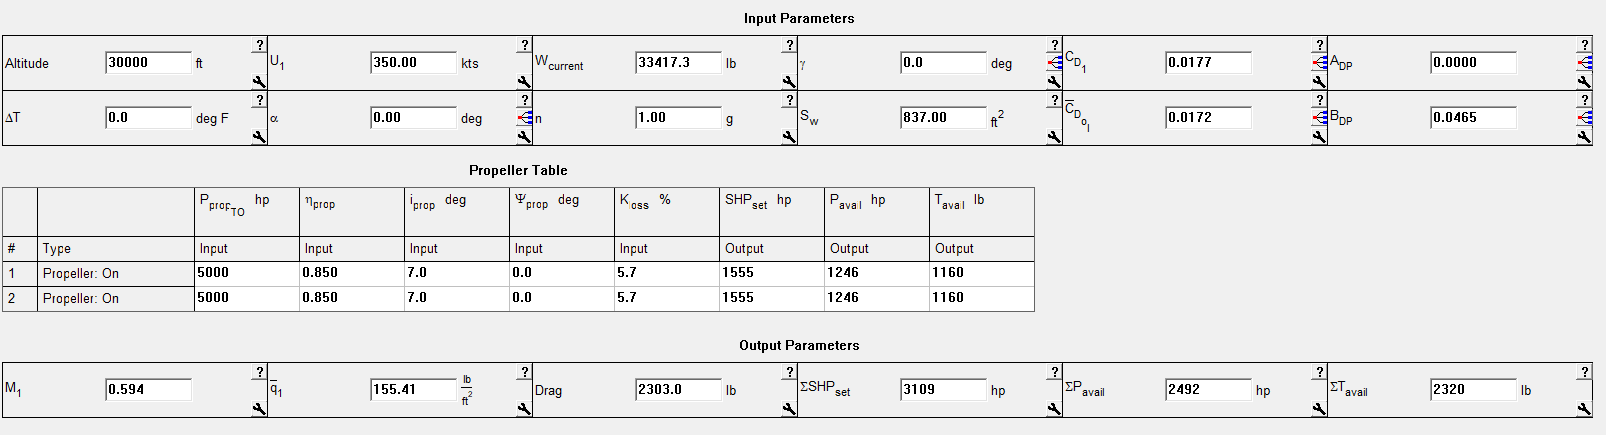
\includegraphics[width=\textwidth]{TwinSeaLionReport2Printouts/enginethrustfromdrag}
	\caption{Engine thrust from drag}
	\label{fig:enginethrustfromdrag}
\end{figure}
%% MOVED TO LIFT SIZING SECTION
%\begin{figure}[H]
%	\centering
%	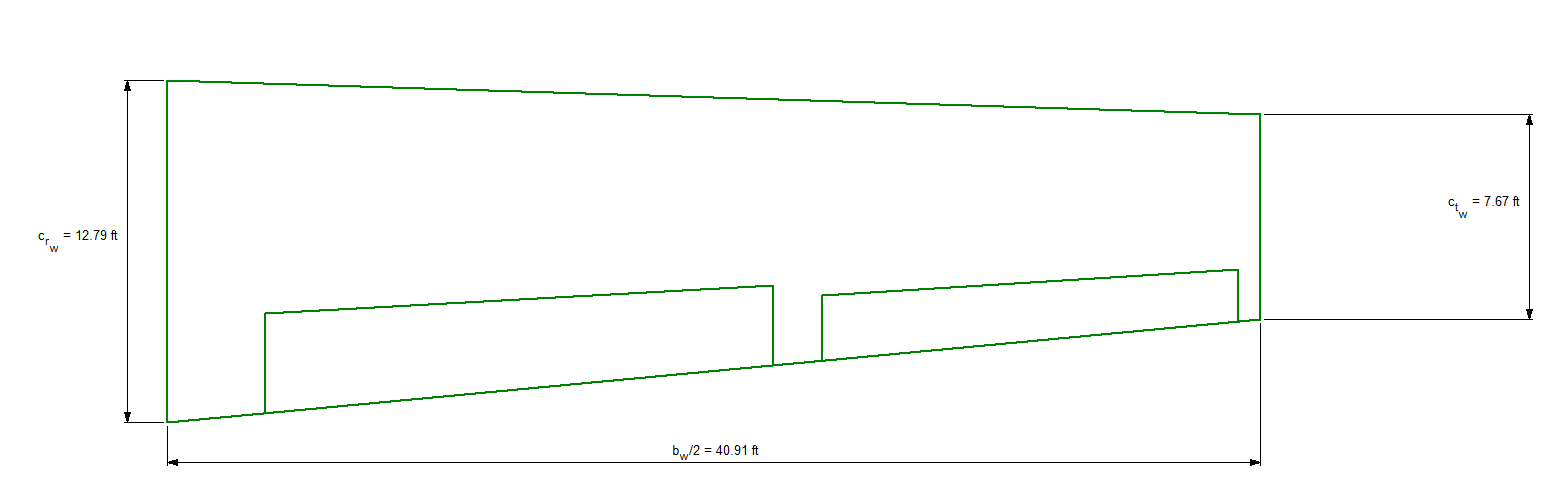
\includegraphics[width=\textwidth]{TwinSeaLionReport2Printouts/HighLiftDeviceSizingPlot}
%	\caption{High lift device sizing plot}
%	\label{fig:HighLiftDeviceSizingPlot}
%\end{figure}
\begin{figure}[H]
	\centering
	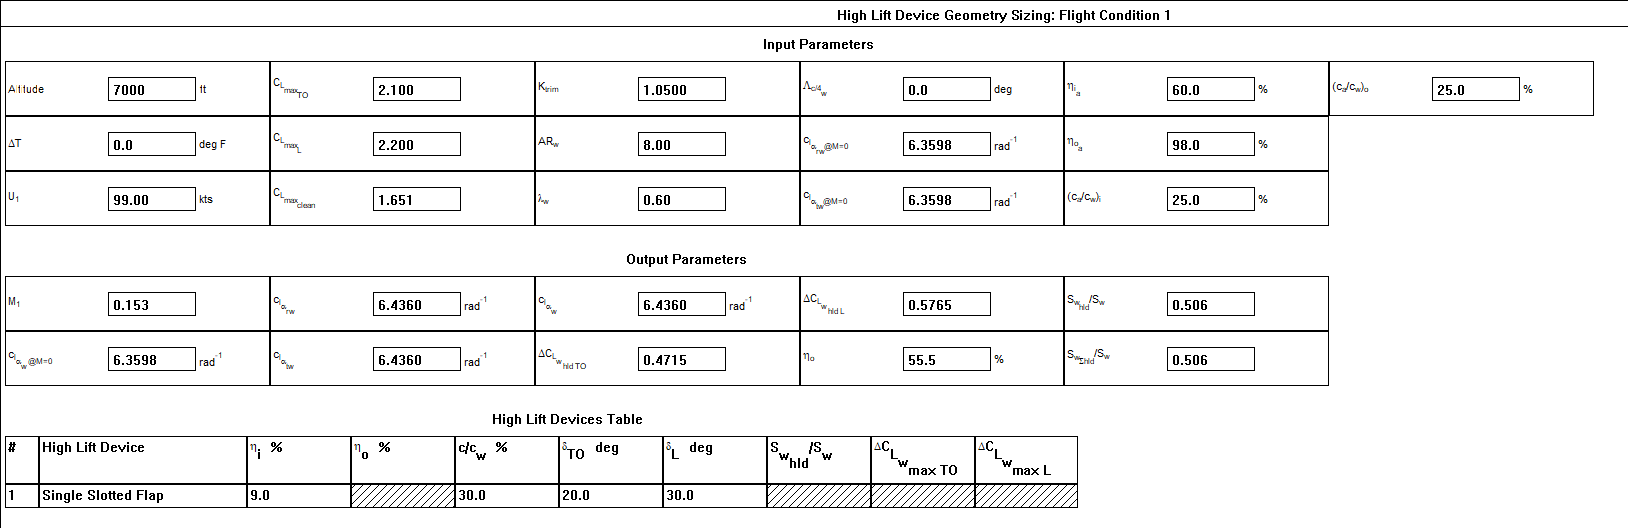
\includegraphics[width=\textwidth]{TwinSeaLionReport2Printouts/HighLiftDeviceSizing}
	\caption{High lift device sizing}
	\label{fig:HighLiftDeviceSizing}
\end{figure}
% \begin{figure}[H]
% 	\centering
% 	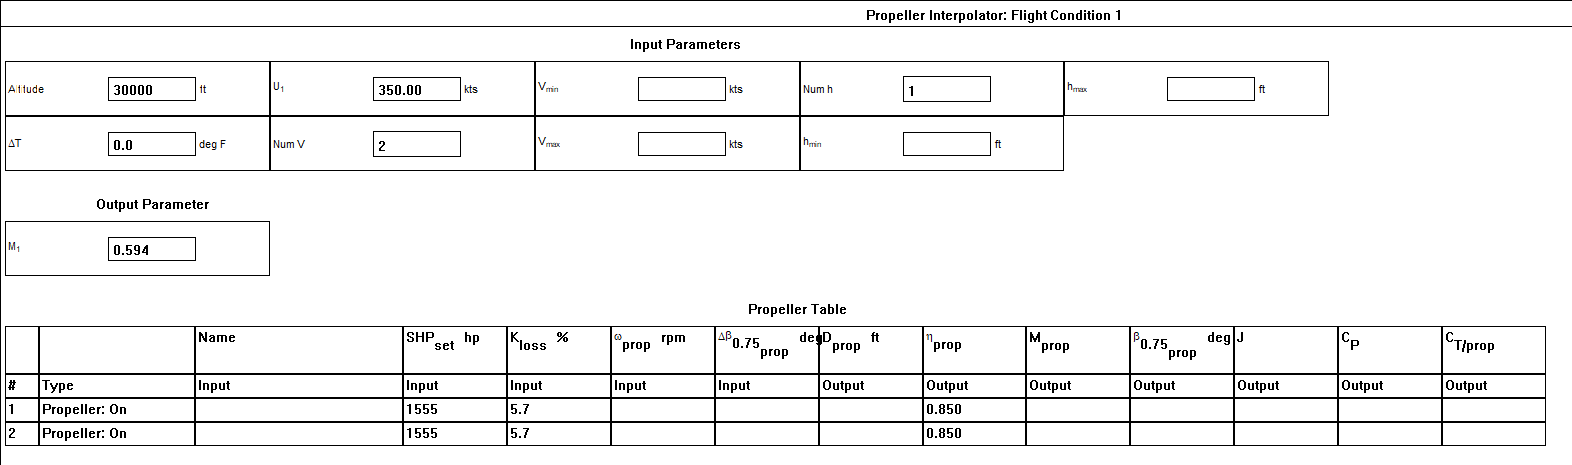
\includegraphics[width=\textwidth]{TwinSeaLionReport2Printouts/propellerInterpolator}
% 	\caption{Propeller interpolator}
% 	\label{fig:propellerInterpolator}
% \end{figure}
% \begin{figure}[H]
% 	\centering
% 	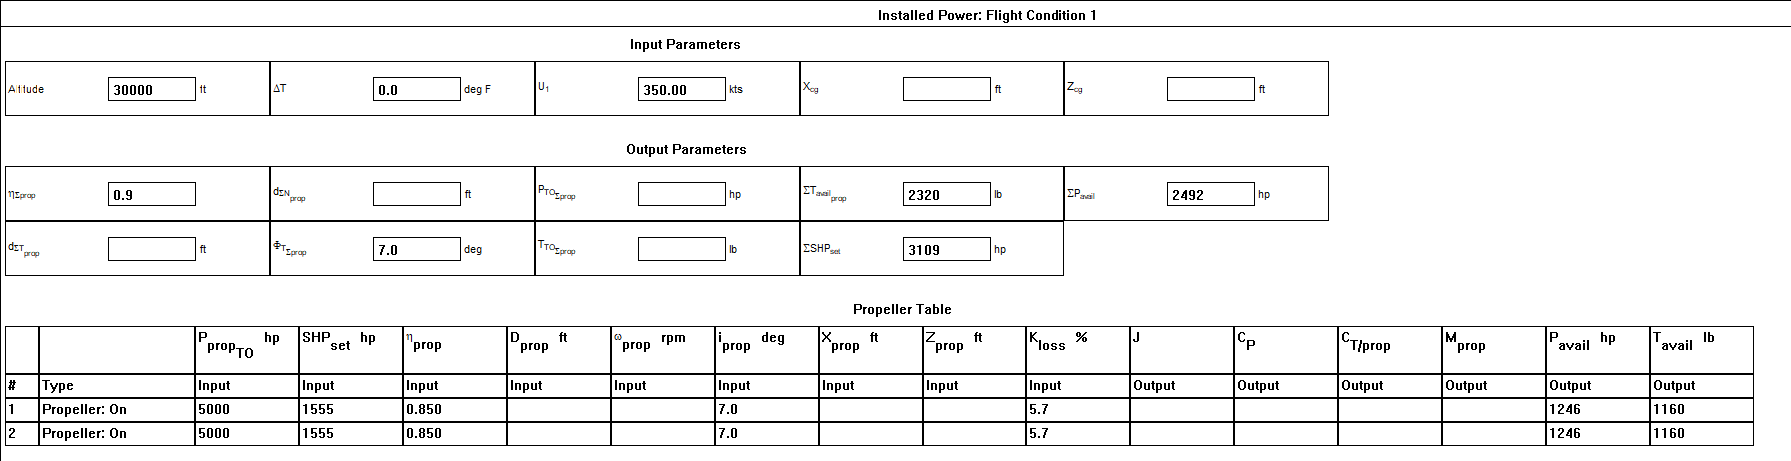
\includegraphics[width=\textwidth]{TwinSeaLionReport2Printouts/propellerPower}
% 	\caption{Propeller power calculations}
% 	\label{fig:propellerPower}
% \end{figure}
%% MOVED TO GEOMETRIC DESIGN
%\begin{figure}[H]
%	\centering
%	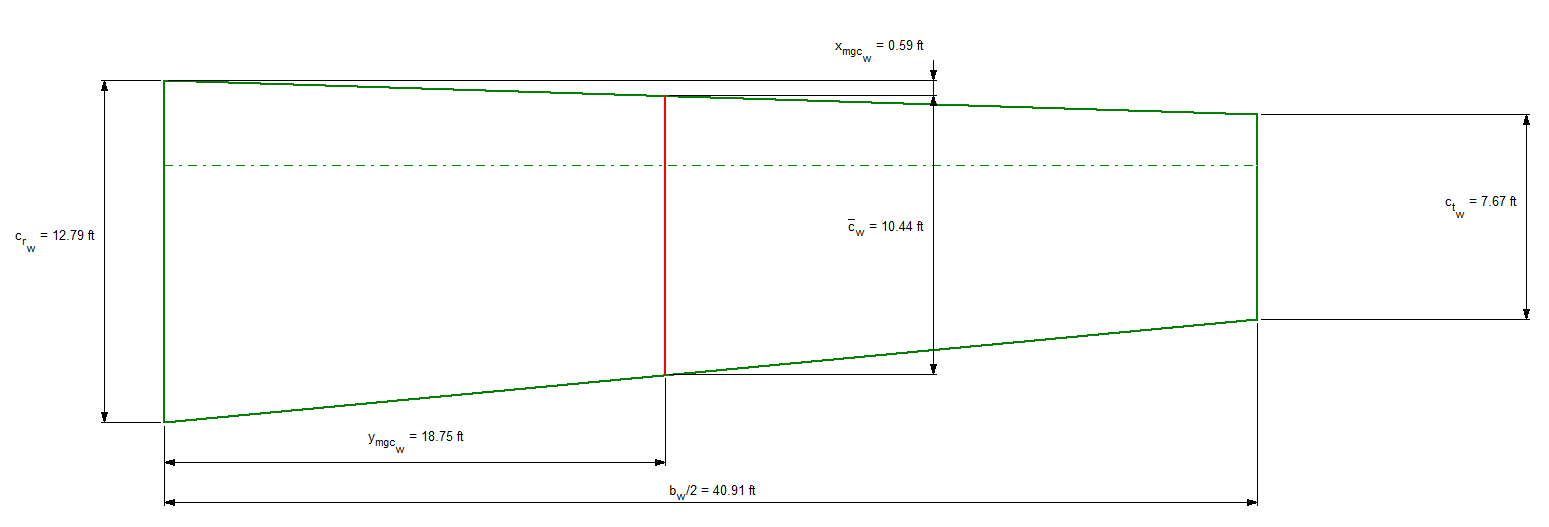
\includegraphics[width=\textwidth]{TwinSeaLionReport2Printouts/StraightTaperedWingGeometryPlot}
%	\caption{Straight tapered wing geometry plot}
%	\label{fig:StraightTaperedWingGeometryPlot}
%\end{figure}
\begin{figure}[H]
	\centering
	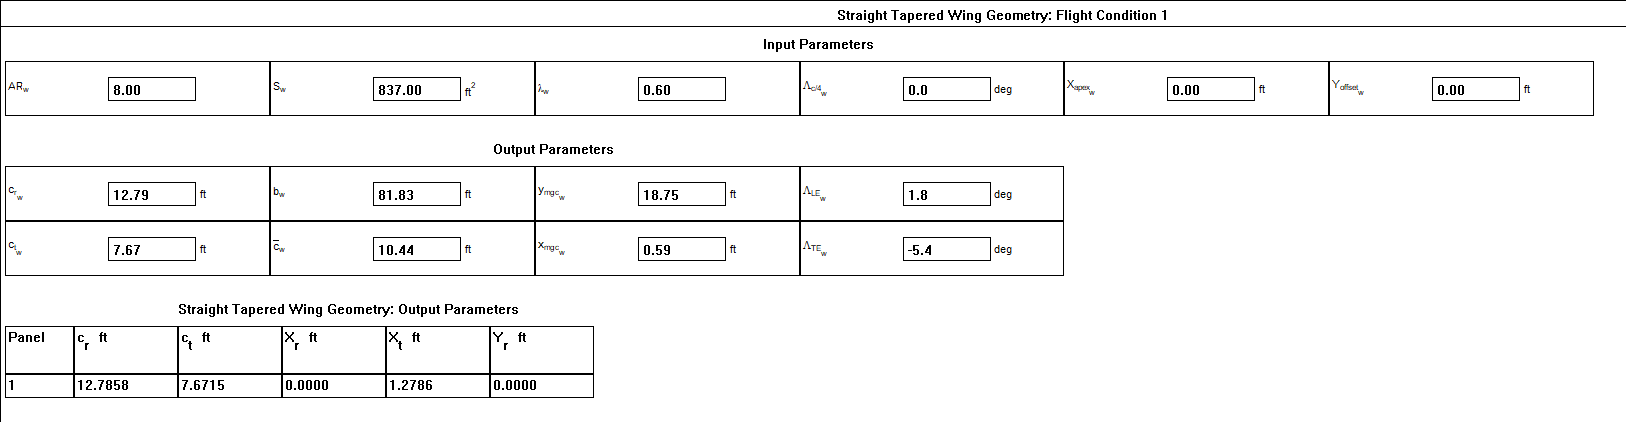
\includegraphics[width=\textwidth]{TwinSeaLionReport2Printouts/StraightTaperedWingGeometry}
	\caption{Straight tapered wing geometry}
	\label{fig:StraightTaperedWingGeometry}
\end{figure}
\begin{figure}[H]
	\centering
	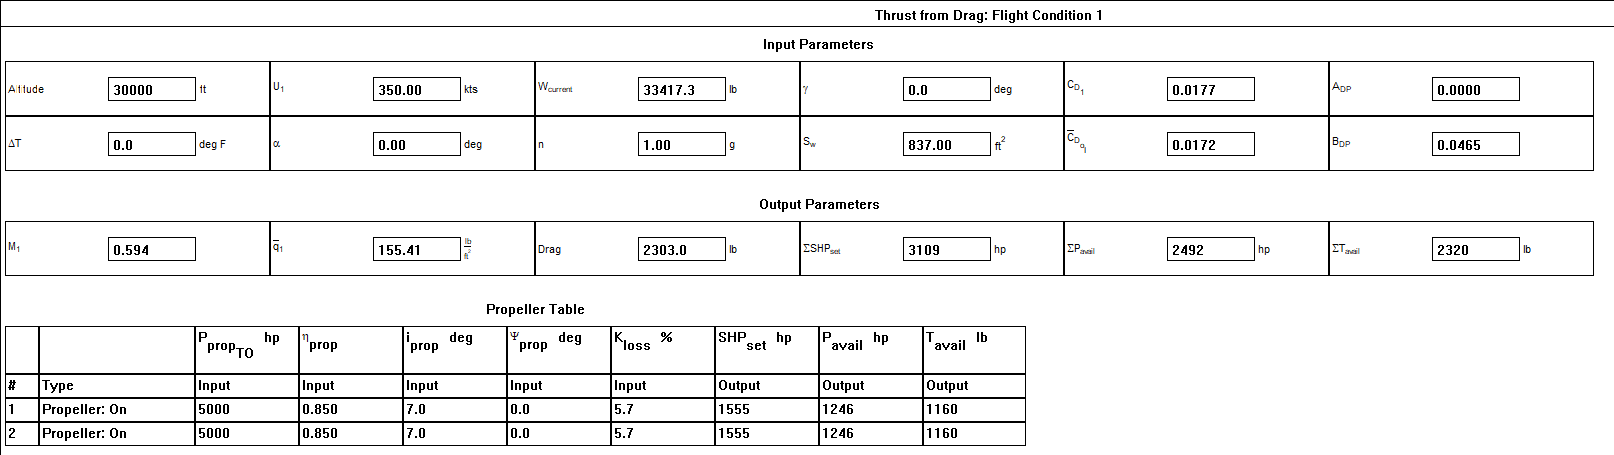
\includegraphics[width=\textwidth]{TwinSeaLionReport2Printouts/thrustFromDrag}
	\caption{Thrust from drag}
	\label{fig:thrustFromDrag}
\end{figure}
\begin{figure}[H]
	\centering
	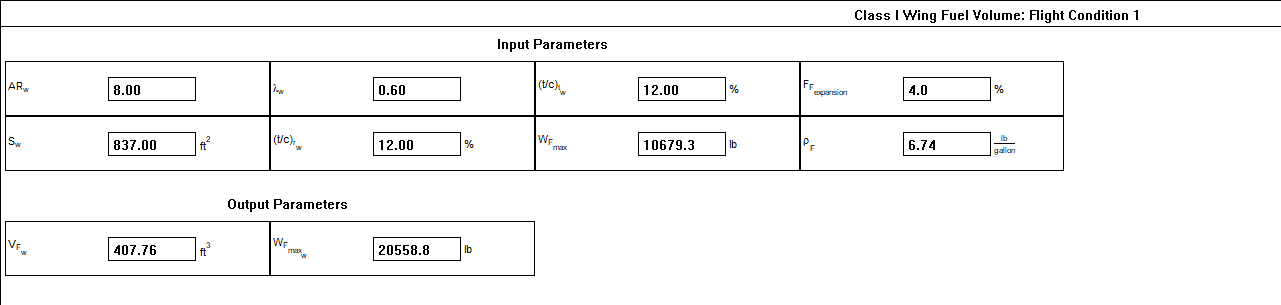
\includegraphics[width=\textwidth]{TwinSeaLionReport2Printouts/WingFuelVolume}
	\caption{Wing fuel volume}
	\label{fig:WingFuelVolume}
\end{figure}
\begin{figure}[H]
	\centering
	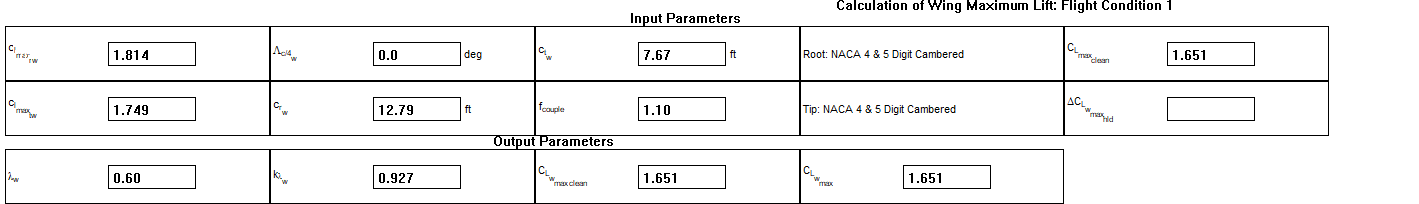
\includegraphics[width=\textwidth]{TwinSeaLionReport2Printouts/WingMaximumLift}
	\caption{Wing maximum lift}
	\label{fig:WingMaximumLift}
\end{figure}

\subsection*{Considered Airfoils and Similar Aircraft}
\begin{table}[H]
    \centering
    \caption{Airfoil options}
    \label{tab:AirfoilOptions}
    \begin{tabular}{|c|c|c|c|c|} \hline
        Name & $C_{l_{max}}$ & $C_{l_{\alpha=0}}$ & $C_{d_{cruise}}$ & In drag Bucket \\ \hline
        NACA 64-110          & 1.4  & 0.1  & 0.004  & yes \\ \hline
        NACA 64-210          & 1.4  & 0.2  & 0.0045 & yes \\ \hline
        NACA 63A010          & 1.2  & 0.0  & 0.0055 & no  \\ \hline
        NACA 63A210          & 1.45 & 0.1  & 0.004  & yes \\ \hline
        NACA 64A210          & 1.4  & 0.15 & 0.004  & yes \\ \hline
        NACA 64A410          & 1.6  & 0.35 & 0.005  & no  \\ \hline
        NACA 65(1)-412       & 1.65 & 0.35 & 0.004  & yes \\ \hline
        NACA 64-110          & 1.4  & 0.1  & 0.004  & yes \\ \hline
        NACA 63A010          & 1.2  & 0.0  & 0.0055 & no  \\ \hline
        Supercritical 2-0714 & 1.75 & 0.6  & 0.006  & yes \\ \hline
        Supercritical 2-0614 & 1.7  & 0.5  & 0.006  & yes \\ \hline
    \end{tabular}
\end{table}

\begin{table}[H]
\centering
\caption{Selected regional turboprop wing geometries}
\label{tab:SelectedWingGeometry}
    \begin{tabular}{|c|c|c|c|c|c|c|c|c|} \hline
        Type             & $\Gamma_W$ (degrees) & $i_w$ (degrees) & $\lambda_W$ \\ \hline
        Shorts 330       & 3   & 0        & 1    \\ \hline
        Shorts 360       & 3   & 0        & 1    \\ \hline
        Beech 1900       & 6   & 3.5/-1.1 & 0.42 \\ \hline
        Beech 99         & 7   & 4.8      & 0.5  \\ \hline
        Fokker F-27      & 2.5 & 3.5      & 0.41 \\ \hline
        DHC-6            & 0   & 0        & 0    \\ \hline
        DHC-7            & 4.5 & 3        & 0.44 \\ \hline
        DHC-8            & 2.5 & 0        & 0.45 \\ \hline
        EMB-110          & 7   & 3        & 0.5  \\ \hline
        EMB-120          & 6.5 & 2        & 0.5  \\ \hline
        BAE Jetstream 31 & 7   & 2        & 0.37 \\ \hline
        BAE 748          & 7   & 3        & 0.37 \\ \hline
    \end{tabular}
\end{table}

\end{document}

